\documentclass[a4paper]{article}
\usepackage{vntex}

\usepackage{a4wide,amssymb,epsfig,latexsym,array,hhline,fancyhdr}
\usepackage[normalem]{ulem}
\usepackage{caption}
\usepackage[makeroom]{cancel}
\usepackage{amsmath}
\usepackage{amsthm}
\usepackage{multicol,longtable,amscd}
\usepackage{diagbox}
\usepackage{booktabs}
\usepackage{alltt}
\usepackage[framemethod=tikz]{mdframed}
\usepackage{caption,subcaption}
\usepackage{minted}
\usepackage{lastpage}
\usepackage[lined,boxed,commentsnumbered]{algorithm2e}
\usepackage{enumerate}
\usepackage{color}
\usepackage{graphicx}
\usepackage{array}
\usepackage{tabularx, caption}
\usepackage{multirow}
\usepackage{multicol}
\usepackage{rotating}
\usepackage{graphics}
\usepackage{geometry}
\usepackage{setspace}
\usepackage{epsfig}
\usepackage{float}
\usepackage{tikz}
\usepackage{pgfplots}
\pgfplotsset{compat=1.18}
\usetikzlibrary{arrows,snakes,backgrounds,positioning,calc,fit}
\usepackage[unicode]{hyperref}
\hypersetup{urlcolor=blue,linkcolor=black,citecolor=black,colorlinks=true}
\usepackage{listings}
\lstset{
    language=Python,
    basicstyle=\ttfamily\small,
    keywordstyle=\color{blue},
    stringstyle=\color{red},
    commentstyle=\color{green},
    morecomment=[l][\color{magenta}]{\#},
    breaklines=true,
    postbreak=\mbox{\textcolor{red}{$\hookrightarrow$}\space},
}
\newcommand{\code}[1]{\texttt{\textcolor{blue!80!black}{#1}}}

\newtheorem{theorem}{{\bf \DJ ịnh lý}}
\newtheorem{property}{{\bf Tính chất}}
\newtheorem{proposition}{{\bf Mệnh đề}}
\newtheorem{corollary}[proposition]{{\bf Hệ quả}}
\newtheorem{lemma}[proposition]{{\bf Bổ đề}}
\theoremstyle{definition}
\newtheorem{exer}{Bài toán}

\def\thesislayout{
	\geometry{
		a4paper,
		total={160mm,240mm},
		left=30mm,
		top=30mm,
	}
}
\thesislayout

\setlength{\headheight}{40pt}
\pagestyle{fancy}
\fancyhead{}
\fancyhead[L]{
 \begin{tabular}{rl}
    \begin{picture}(25,15)(0,0)
    \put(0,-8){
\includegraphics[width=8mm, height=8mm]{Images/hcmut.png}}
   \end{picture}&
	\begin{tabular}{l}
		\textbf{\bf \ttfamily Trường \DJ ại Học Bách Khoa Tp.Hồ Chí Minh}\\
		\textbf{\bf \ttfamily Khoa Khoa Học \& Kỹ Thuật Máy Tính}
	\end{tabular}
 \end{tabular}
}
\fancyhead[R]{
	\begin{tabular}{l}
		\tiny \bf \\
		\tiny \bf
	\end{tabular}  }
\fancyfoot{}
\fancyfoot[L]{\scriptsize \ttfamily Bài tập môn Học sâu và ứng dụng trong thị giác máy tính - Niên khóa 2025-2026}
\fancyfoot[R]{\scriptsize \ttfamily Trang {\thepage}/\pageref{LastPage}}
\renewcommand{\headrulewidth}{0.3pt}
\renewcommand{\footrulewidth}{0.3pt}

\setcounter{secnumdepth}{4}
\setcounter{tocdepth}{3}
\makeatletter
\newcounter {subsubsubsection}[subsubsection]
\renewcommand\thesubsubsubsection{\thesubsubsection .\arabic{subsubsubsection}}
\newcommand\subsubsubsection{\@startsection{subsubsubsection}{4}{\z@}%
                                     {-3.25ex\@plus -1ex \@minus -.2ex}%
                                     {1.5ex \@plus .2ex}%
                                     {\normalfont\normalsize\bfseries}}
\newcommand*\l@subsubsubsection{\@dottedtocline{3}{10.0em}{4.1em}}
\newcommand*{\subsubsubsectionmark}[1]{}
\makeatother

\sloppy
\captionsetup[figure]{labelfont={small,bf},textfont={small,it},belowskip=-1pt,aboveskip=-9pt}
\captionsetup[table]{labelfont={small,bf},textfont={small,it},belowskip=-1pt,aboveskip=7pt}

\setlength{\floatsep}{5pt plus 2pt minus 2pt}
\setlength{\textfloatsep}{5pt plus 2pt minus 2pt}
\setlength{\intextsep}{10pt plus 2pt minus 2pt}

\thesislayout

\begin{document}

\begin{titlepage}
	\begin{center}
		\DJ ẠI HỌC QUỐC GIA THÀNH PHỐ HỒ CHÍ MINH \\
		TRƯỜNG \DJ ẠI HỌC BÁCH KHOA \\
		KHOA KHOA HỌC \& KỸ THUẬT MÁY TÍNH
	\end{center}

	\vspace{1cm}

	\begin{figure}[h!]
		\begin{center}
			
\includegraphics[width=3cm]{Images/hcmut.png}
		\end{center}
	\end{figure}

	\vspace{1cm}

	\begin{center}
		\begin{tabular}{c}
			\multicolumn{1}{l}{\textbf{{\Large HỌC SÂU VÀ ỨNG DỤNG TRONG THỊ GIÁC MÁY TÍNH}}} \\
			~~                                                                                \\
			\hline
			\\
			\multicolumn{1}{l}{\textbf{{\large Bài tập -- Nhóm 4}}}                   \\
			\textbf{\Large Phân loại ảnh với các mô hình học sâu cơ bản}                                                  \\
			\\
			\hline
		\end{tabular}
	\end{center}

	\vspace{1.5cm}

	\begin{table}[h]
		\begin{tabular}{rrl}
			\hspace{5 cm} & GVHD:         & TS. Lê Thành Sách            \\

			              & SV thực hiện: & Nguyễn Hữu Trưởng - 2470573  \\
			              &               & Nguyễn Nhật Thanh - 2570316  \\
			              &               & Võ Thị Bích Phượng - 2470570 \\
		\end{tabular}
	\end{table}
	\vspace{1.5cm}
	\begin{center}
		\vfill
		{\footnotesize Tp. Hồ Chí Minh, Tháng 03/2026}
	\end{center}
\end{titlepage}

\newpage
\tableofcontents
\newpage

%%%%%%%%%%%%%%%%%%%%%%%%%%%%%%%%%
% PHẦN 1: GIỚI THIỆU
%%%%%%%%%%%%%%%%%%%%%%%%%%%%%%%%%
\section{Giới thiệu}

\subsection{Mục tiêu bài tập}
Bài tập này thuộc môn \textbf{Học sâu và ứng dụng trong thị giác máy tính} (mã môn học: CO5085), năm học 2025--2026, Học kỳ 2. Mục tiêu chính là giúp sinh viên nắm vững \textbf{cơ bản về học sâu và ứng dụng trong thị giác máy tính} thông qua việc:

\begin{itemize}
	\item Xây dựng và so sánh các mô hình phân loại ảnh từ đơn giản đến phức tạp: \textbf{Softmax Regression}, \textbf{MLP}, \textbf{CNN}, \textbf{Vision Transformer (ViT)}, và mô hình dựa trên \textbf{LSTM/GRU}.
	\item Tự viết vòng lặp huấn luyện (training loop) bằng PyTorch, sử dụng \code{backward} có sẵn để tính đạo hàm, thay vì chỉ gọi API cấp cao.
	\item Hiểu cấu trúc bên trong Transformer qua việc tự hiện thực khối \code{TransformerEncoder} từ các phép toán cơ bản.
	\item Khám phá các cách thiết kế kiến trúc khác nhau: kết hợp CNN--Transformer, các cách tokenize/embed ảnh khác nhau, và biểu diễn ảnh thành chuỗi cho RNN.
\end{itemize}

\subsection{Nội dung bài tập}
Theo yêu cầu đề bài, bài tập được chia thành 5 phần chính:

\begin{enumerate}
	\item \textbf{Phần 1 -- Xây dựng các mô hình phân loại:} Xây dựng lần lượt bốn mô hình Softmax Regression, MLP, CNN và ViT (sử dụng khối có sẵn của PyTorch) cho bài toán phân loại ảnh trên tập dữ liệu CIFAR-10.

	\item \textbf{Phần 2 -- Huấn luyện, đánh giá và so sánh:} Tự viết giải thuật huấn luyện (training loop) dựa trên PyTorch với vòng lặp theo epoch/batch, gọi \code{loss.backward()} và cập nhật tham số bằng optimizer. Sử dụng vòng lặp này để huấn luyện, đánh giá và so sánh bốn mô hình ở Phần 1.

	\item \textbf{Phần 3 -- Tự hiện thực TransformerEncoder và ViT:} Tự hiện thực khối \code{TransformerEncoder} từ các phép toán cơ bản của PyTorch (Linear, LayerNorm, einsum), \textit{không} dùng \code{nn.TransformerEncoderLayer} hay \code{nn.TransformerEncoder} có sẵn. Xây dựng ViT dựa trên khối tự hiện thực và so sánh với ViT dùng khối có sẵn ở Phần 1.

	\item \textbf{Phần 4 -- Các kiến trúc kết hợp và cách embed ảnh khác nhau:} Xây dựng các kiến trúc lai như \textbf{Hybrid CNN + Transformer} (dùng CNN làm backbone trích đặc trưng rồi đưa vào Transformer) và \textbf{Overlapping Patches ViT} (dùng patch chồng mép để tạo token).

	\item \textbf{Phần 5 -- Mô hình phân loại dựa trên LSTM/GRU:} Xây dựng mô hình phân loại dựa trên LSTM và GRU, tự chọn cách biểu diễn ảnh thành chuỗi (sequence). So sánh LSTM vs GRU trên cùng cách biểu diễn.
\end{enumerate}

\subsection{Tập dữ liệu và Công cụ}
Nhóm lựa chọn tập dữ liệu \textbf{CIFAR-10} gồm 60.000 ảnh màu RGB kích thước $32 \times 32$ pixel, phân bổ đều vào 10 lớp. Toàn bộ thực nghiệm được hiện thực bằng \textbf{PyTorch} và huấn luyện trên GPU NVIDIA Tesla T4.

\subsection{Cấu trúc báo cáo}
Báo cáo được tổ chức theo thứ tự từ mô hình đơn giản đến phức tạp: Softmax Regression $\to$ MLP $\to$ CNN $\to$ ViT $\to$ Custom ViT $\to$ Hybrid CNN-Transformer $\to$ Overlapping ViT $\to$ LSTM/GRU. Mỗi phần bao gồm: giới thiệu lý thuyết, kiến trúc mô hình, công thức toán học, mã nguồn hiện thực, cấu hình huấn luyện, và kết quả thực nghiệm. Cuối cùng là phần so sánh tổng hợp và nhận xét.

%%%%%%%%%%%%%%%%%%%%%%%%%%%%%%%%%
% PHẦN 2: TẬP DỮ LIỆU CIFAR-10
%%%%%%%%%%%%%%%%%%%%%%%%%%%%%%%%%
\section{Tập dữ liệu CIFAR-10 và Tiền xử lý}

\subsection{Giới thiệu tập dữ liệu CIFAR-10}
CIFAR-10 (Canadian Institute For Advanced Research) \cite{krizhevsky2009learning} là một trong những tập dữ liệu chuẩn (benchmark) phổ biến nhất trong lĩnh vực thị giác máy tính. Tập dữ liệu bao gồm \textbf{60.000 ảnh màu RGB} có kích thước $32 \times 32$ pixel, phân bổ \textbf{đều} vào 10 lớp (mỗi lớp 6.000 ảnh):

\begin{center}
\textit{airplane, automobile, bird, cat, deer, dog, frog, horse, ship, truck}
\end{center}

Tập dữ liệu được chia sẵn thành 50.000 ảnh huấn luyện (training) và 10.000 ảnh kiểm thử (test). Phân bố các lớp hoàn toàn cân bằng với 5.000 ảnh mỗi lớp trong tập huấn luyện.

\begin{figure}[H]
	\centering
	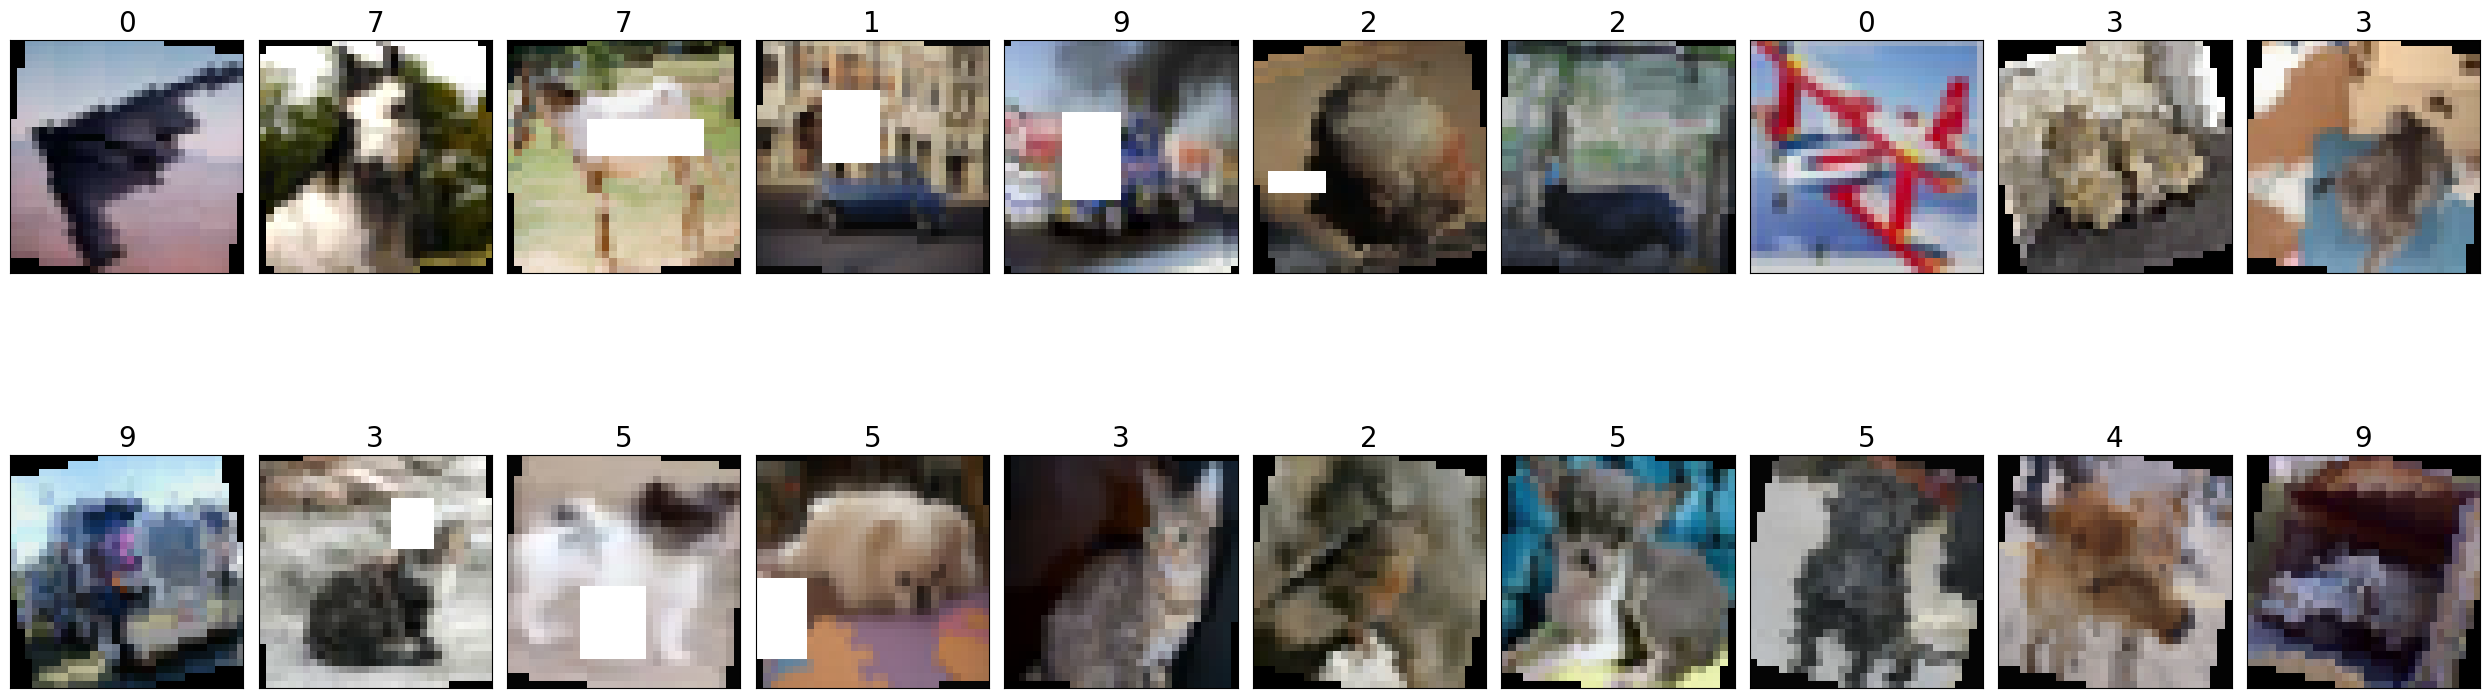
\includegraphics[width=0.65\linewidth]{Images/cifar10.png}
	\vspace{10pt}
	\caption{Ảnh mẫu từ 10 lớp trong tập dữ liệu CIFAR-10}
	\label{fig:cifar10}
\end{figure}

\subsection{Phân chia dữ liệu}

\subsubsection{Cho các mô hình Softmax, MLP, CNN, ViT và các biến thể}
Từ tập huấn luyện gốc 50.000 ảnh, nhóm chia thành hai phần bằng \code{random\_split} với \code{seed=42}:

\begin{table}[H]
	\centering
	\caption{Phân chia dữ liệu cho các mô hình CNN/ViT}
	\begin{tabular}{|l|c|c|l|}
		\hline
		\textbf{Tập dữ liệu} & \textbf{Số lượng} & \textbf{Tỷ lệ} & \textbf{Mục đích} \\ \hline
		Training Set          & 40.000            & 80\%           & Huấn luyện mô hình \\ \hline
		Validation Set        & 10.000            & 20\%           & Theo dõi hiệu suất, chọn mô hình tốt nhất \\ \hline
		Test Set              & 10.000            & --             & \DJ ánh giá cuối cùng (tập độc lập) \\ \hline
	\end{tabular}
	\label{tab:data-split-cnn}
\end{table}

\subsubsection{Cho các mô hình LSTM/GRU}
Do huấn luyện trên notebook riêng với cấu hình khác, tập dữ liệu được chia:

\begin{table}[H]
	\centering
	\caption{Phân chia dữ liệu cho các mô hình LSTM/GRU}
	\begin{tabular}{|l|c|c|l|}
		\hline
		\textbf{Tập dữ liệu} & \textbf{Số lượng} & \textbf{Tỷ lệ} & \textbf{Mục đích} \\ \hline
		Training Set          & 45.000            & 90\%           & Huấn luyện mô hình \\ \hline
		Validation Set        & 5.000             & 10\%           & Theo dõi hiệu suất \\ \hline
		Test Set              & 10.000            & --             & \DJ ánh giá cuối cùng \\ \hline
	\end{tabular}
	\label{tab:data-split-rnn}
\end{table}

\subsection{Tiền xử lý dữ liệu (Data Preprocessing)}

\subsubsection{Bộ transform cho mạng tự xây dựng (32$\times$32)}
Các mô hình Softmax, MLP, CNN, ViT và các biến thể sử dụng ảnh gốc $32 \times 32$ pixel với chuẩn hóa về khoảng $[-1, 1]$. Riêng tập huấn luyện được áp dụng thêm các kỹ thuật tăng cường dữ liệu (data augmentation):

\begin{minted}[linenos, breaklines, fontsize=\small]{python}
train_transform_custom = transforms.Compose([
    transforms.RandomRotation(15),
    transforms.RandomHorizontalFlip(p=0.5),
    transforms.ColorJitter(brightness=0.1, contrast=0.1, saturation=0.1),
    transforms.RandomAdjustSharpness(sharpness_factor=2, p=0.1),
    transforms.ToTensor(),
    transforms.Normalize((0.5, 0.5, 0.5), (0.5, 0.5, 0.5)),
    transforms.RandomErasing(p=0.5, scale=(0.02, 0.1), value=1.0)
])

test_transform_custom = transforms.Compose([
    transforms.ToTensor(),
    transforms.Normalize((0.5, 0.5, 0.5), (0.5, 0.5, 0.5))
])
\end{minted}

Các kỹ thuật tăng cường bao gồm: xoay ngẫu nhiên (RandomRotation $15\degree$), lật ngang ngẫu nhiên (RandomHorizontalFlip), biến đổi màu sắc (ColorJitter), điều chỉnh độ nét (RandomAdjustSharpness), và xóa ngẫu nhiên (RandomErasing). Mục đích là tăng tính đa dạng của dữ liệu huấn luyện, giúp mô hình tổng quát hóa tốt hơn.

\subsubsection{Bộ transform cho mô hình LSTM/GRU}
Các mô hình LSTM/GRU sử dụng chuẩn hóa theo giá trị trung bình và độ lệch chuẩn thực tế của CIFAR-10, \textit{không} áp dụng data augmentation:

\begin{minted}[linenos, breaklines, fontsize=\small]{python}
transform = transforms.Compose([
    transforms.ToTensor(),
    transforms.Normalize(
        mean=(0.4914, 0.4822, 0.4465),  # Mean cua CIFAR-10
        std=(0.2470, 0.2435, 0.2616)    # Std cua CIFAR-10
    )
])
\end{minted}

\subsection{Hàm huấn luyện và đánh giá chung}
Nhóm xây dựng một hàm huấn luyện chung \code{train\_and\_evaluate} cho tất cả các mô hình (trừ LSTM/GRU), bao gồm các thành phần:

\begin{itemize}
	\item \textbf{Hàm mất mát:} \code{CrossEntropyLoss} (đã tích hợp Softmax bên trong).
	\item \textbf{Thuật toán tối ưu:} Adam.
	\item \textbf{Scheduler:} \code{ReduceLROnPlateau} -- giảm learning rate đi một nửa khi validation loss không cải thiện sau 2 epoch.
	\item \textbf{Early Stopping:} Dừng huấn luyện sớm khi validation loss không cải thiện sau một số epoch nhất định (patience), đồng thời lưu checkpoint tốt nhất.
\end{itemize}

\begin{minted}[linenos, breaklines, fontsize=\small]{python}
def train_and_evaluate(model_name, model, train_loader, val_loader,
                       epochs, lr, device, patience=5, save_path=None):
    criterion = nn.CrossEntropyLoss()
    optimizer = optim.Adam(model.parameters(), lr=lr)
    scheduler = optim.lr_scheduler.ReduceLROnPlateau(
        optimizer, mode='min', factor=0.5, patience=2)

    best_val_loss = float('inf')
    epochs_no_improve = 0

    for epoch in range(epochs):
        # --- TRAIN ---
        model.train()
        for inputs, labels in train_loader:
            inputs, labels = inputs.to(device), labels.to(device)
            optimizer.zero_grad()
            outputs = model(inputs)
            loss = criterion(outputs, labels)
            loss.backward()
            optimizer.step()

        # --- VALIDATE ---
        model.eval()
        with torch.no_grad():
            # Tinh val_loss, val_acc ...
            pass

        scheduler.step(val_loss)

        if val_loss < best_val_loss:
            best_val_loss = val_loss
            epochs_no_improve = 0
            torch.save(model.state_dict(), save_path)
        else:
            epochs_no_improve += 1
            if epochs_no_improve >= patience:
                break  # Early stopping

    model.load_state_dict(torch.load(save_path))
    return history
\end{minted}

%%%%%%%%%%%%%%%%%%%%%%%%%%%%%%%%%
% PHẦN 3: SOFTMAX REGRESSION
%%%%%%%%%%%%%%%%%%%%%%%%%%%%%%%%%
\section{Hồi quy Softmax (Softmax Regression)}

\subsection{Giới thiệu}
Hồi quy Softmax (Softmax Regression), còn gọi là hồi quy logistic đa lớp (Multinomial Logistic Regression), là mô hình phân loại tuyến tính đơn giản nhất cho bài toán phân loại nhiều lớp. Mô hình này ánh xạ trực tiếp vector đầu vào thành phân phối xác suất trên các lớp, \textit{không} sử dụng bất kỳ lớp ẩn nào.

\subsection{Kiến trúc và Công thức toán học}

\subsubsection{Mô hình tuyến tính}
Cho vector đầu vào $\mathbf{x} \in \mathbb{R}^d$ (ảnh đã được flatten), mô hình tính \textit{logits} (điểm số thô) cho mỗi lớp $k$:
\begin{equation}
	z_k = \mathbf{w}_k^T \mathbf{x} + b_k, \quad k = 1, 2, \ldots, K
	\label{eq:softmax-logits}
\end{equation}
trong đó $\mathbf{w}_k \in \mathbb{R}^d$ là vector trọng số và $b_k$ là hệ số chệch của lớp $k$, $K=10$ là số lớp.

Viết dưới dạng ma trận: $\mathbf{z} = W\mathbf{x} + \mathbf{b}$ với $W \in \mathbb{R}^{K \times d}$, $\mathbf{b} \in \mathbb{R}^K$.

\subsubsection{Hàm Softmax}
\DJ ể chuyển logits thành phân phối xác suất, hàm \textbf{Softmax} được áp dụng:
\begin{equation}
	P(y = k \mid \mathbf{x}) = \text{softmax}(z_k) = \frac{e^{z_k}}{\sum_{j=1}^{K} e^{z_j}}
	\label{eq:softmax-func}
\end{equation}

Hàm Softmax đảm bảo: (1) mọi xác suất đều dương $P(y=k|\mathbf{x}) > 0$, và (2) tổng xác suất bằng 1: $\sum_k P(y=k|\mathbf{x}) = 1$.

\subsubsection{Hàm mất mát Cross-Entropy}
Hàm mất mát Cross-Entropy đo khoảng cách giữa phân phối dự đoán và nhãn thật (one-hot encoding):
\begin{equation}
	\mathcal{L} = -\sum_{k=1}^{K} y_k \log P(y = k \mid \mathbf{x}) = -\log P(y = c \mid \mathbf{x})
	\label{eq:cross-entropy}
\end{equation}
trong đó $c$ là lớp đúng của mẫu. Trong PyTorch, \code{nn.CrossEntropyLoss} đã tích hợp sẵn cả hàm Softmax và Cross-Entropy, nên mô hình chỉ cần trả về logits.

\subsection{\DJ ặc điểm của mô hình}
\begin{itemize}
	\item \textbf{Ưu điểm:} \DJ ơn giản, ít tham số, dễ hiểu, huấn luyện nhanh. Là baseline tốt để so sánh.
	\item \textbf{Nhược điểm:} Chỉ học được ranh giới phân loại tuyến tính (linear decision boundary), không thể nắm bắt các mối quan hệ phi tuyến hay đặc trưng không gian (spatial features) trong ảnh. Việc flatten ảnh thành vector 1D làm mất hoàn toàn cấu trúc không gian 2D.
\end{itemize}

\subsection{Áp dụng cho bài tập}

\subsubsection{Kiến trúc mô hình}
Ảnh CIFAR-10 có kích thước $3 \times 32 \times 32 = 3072$ pixel. Mô hình gồm hai bước:
\begin{enumerate}
	\item \textbf{Flatten:} Biến ảnh $(B, 3, 32, 32)$ thành vector $(B, 3072)$.
	\item \textbf{Linear:} Ánh xạ tuyến tính $\text{Linear}(3072, 10)$ cho 10 lớp.
\end{enumerate}

\textbf{Tổng số tham số:} $3072 \times 10 + 10 = 30.730$

\subsubsection{Mã nguồn}
\begin{minted}[linenos, breaklines, fontsize=\small]{python}
class SoftmaxRegression(nn.Module):
    def __init__(self):
        super(SoftmaxRegression, self).__init__()
        self.flatten = nn.Flatten()
        self.linear = nn.Linear(in_features=32*32*3, out_features=10)

    def forward(self, x):
        x = self.flatten(x)       # (B, 3, 32, 32) -> (B, 3072)
        logits = self.linear(x)   # (B, 3072) -> (B, 10)
        return logits
\end{minted}

\subsubsection{Cấu hình huấn luyện}
\begin{table}[H]
	\centering
	\caption{Cấu hình huấn luyện Softmax Regression}
	\begin{tabular}{|l|c|}
		\hline
		\textbf{Thông số}          & \textbf{Giá trị} \\ \hline
		Optimizer                  & Adam (weight\_decay=$10^{-4}$) \\ \hline
		Learning Rate              & $10^{-3}$ \\ \hline
		Batch Size                 & 512 \\ \hline
		Max Epochs                 & 100 \\ \hline
		Early Stopping Patience    & 5 \\ \hline
		LR Scheduler               & ReduceLROnPlateau (factor=0.5, patience=2) \\ \hline
		Data Augmentation          & Có (transform\_custom) \\ \hline
	\end{tabular}
	\label{tab:softmax-config}
\end{table}

\subsection{Kết quả thực nghiệm}

Mô hình dừng huấn luyện sớm tại \textbf{Epoch 24} do early stopping. Learning rate được giảm tự động từ $10^{-3}$ xuống $1.25 \times 10^{-4}$ qua nhiều lần kích hoạt scheduler.

\begin{table}[H]
	\centering
	\caption{Kết quả huấn luyện Softmax Regression qua các epoch đáng chú ý}
	\footnotesize
	\begin{tabular}{|c|c|c|c|c|c|}
		\hline
		\textbf{Epoch} & \textbf{LR} & \textbf{Train Loss} & \textbf{Train Acc (\%)} & \textbf{Val Loss} & \textbf{Val Acc (\%)} \\ \hline
		1   & $10^{-3}$          & 1.9177 & 32.26 & 1.8420 & 35.64 \\ \hline
		10  & $10^{-3}$          & 1.7955 & 38.02 & 1.7916 & 37.92 \\ \hline
		14  & $5 \times 10^{-4}$ & 1.7776 & 38.88 & 1.7734 & 39.20 \\ \hline
		19  & $2.5 \times 10^{-4}$ & 1.7592 & 39.74 & \textbf{1.7565} & 39.90 \\ \hline
		24  & $1.25 \times 10^{-4}$ & 1.7520 & 40.19 & 1.7569 & \textbf{40.04} \\ \hline
	\end{tabular}
	\label{tab:softmax-results}
\end{table}

\begin{itemize}
	\item \textbf{Best Validation Loss:} 1.7565 tại Epoch 19.
	\item \textbf{Best Validation Accuracy:} 40.04\% tại Epoch 24.
	\item \textbf{Test Accuracy:} $\mathbf{40.89\%}$.
\end{itemize}

\subsection{Nhận xét}
Với Test Accuracy chỉ đạt $40.89\%$ (gần ngẫu nhiên là $10\%$ cho 10 lớp), mô hình Softmax Regression cho thấy những hạn chế rõ ràng:
\begin{itemize}
	\item Ranh giới phân loại tuyến tính không đủ phức tạp để phân biệt 10 lớp ảnh có sự tương đồng cao (ví dụ: cat vs dog, automobile vs truck).
	\item Việc flatten ảnh thành vector 1D phá hủy hoàn toàn cấu trúc không gian, khiến mô hình không thể khai thác thông tin về vị trí tương đối giữa các pixel.
	\item Khoảng cách giữa Train Accuracy ($40.19\%$) và Val Accuracy ($40.04\%$) rất nhỏ, cho thấy mô hình \textit{không} bị quá khớp mà đơn giản là \textit{thiếu năng lực biểu diễn} (underfitting).
\end{itemize}

%%%%%%%%%%%%%%%%%%%%%%%%%%%%%%%%%
% PHẦN 4: MLP
%%%%%%%%%%%%%%%%%%%%%%%%%%%%%%%%%
\section{Mạng Perceptron \DJ a tầng (MLP)}

\subsection{Giới thiệu}
Mạng Perceptron \DJ a tầng (Multi-Layer Perceptron -- MLP) là sự mở rộng tự nhiên của Softmax Regression bằng cách thêm một hoặc nhiều \textit{lớp ẩn} (hidden layers) với hàm kích hoạt phi tuyến. Nhờ đó, MLP có khả năng học các ranh giới phân loại phi tuyến phức tạp hơn.

Theo \textbf{Định lý Xấp xỉ Tổng quát} (Universal Approximation Theorem) \cite{hornik1989multilayer}, một MLP chỉ với một lớp ẩn đủ rộng có thể xấp xỉ bất kỳ hàm liên tục nào với độ chính xác tùy ý. Tuy nhiên trên thực tế, mạng sâu hơn (nhiều lớp hẹp hơn) thường hiệu quả hơn mạng nông rộng.

\subsection{Kiến trúc và Công thức toán học}

\subsubsection{Cấu trúc MLP}
Một MLP gồm $L$ lớp ẩn thực hiện chuỗi biến đổi:
\begin{equation}
	\mathbf{h}^{(l)} = \phi\left(W^{(l)} \mathbf{h}^{(l-1)} + \mathbf{b}^{(l)}\right), \quad l = 1, 2, \ldots, L
	\label{eq:mlp-hidden}
\end{equation}
trong đó $\mathbf{h}^{(0)} = \mathbf{x}$ là đầu vào (ảnh đã flatten), $W^{(l)}$ và $\mathbf{b}^{(l)}$ là trọng số và bias của lớp $l$, $\phi$ là hàm kích hoạt phi tuyến.

Lớp đầu ra tính logits: $\mathbf{z} = W^{(L+1)} \mathbf{h}^{(L)} + \mathbf{b}^{(L+1)}$

\subsubsection{Hàm kích hoạt ReLU}
Hàm kích hoạt \textbf{ReLU} (Rectified Linear Unit) được sử dụng phổ biến nhất:
\begin{equation}
	\text{ReLU}(x) = \max(0, x)
	\label{eq:relu}
\end{equation}
ReLU đơn giản, tính toán nhanh, và giúp giảm thiểu vấn đề triệt tiêu đạo hàm so với sigmoid hay tanh.

\subsubsection{Kỹ thuật điều chuẩn (Regularization)}
\DJ ể chống quá khớp, nhóm sử dụng hai kỹ thuật:

\textbf{Dropout} \cite{srivastava2014dropout}: Tắt ngẫu nhiên một tỷ lệ $p$ các neuron trong quá trình huấn luyện, buộc mạng không phụ thuộc vào bất kỳ neuron đơn lẻ nào:
\begin{equation}
	\hat{\mathbf{h}}^{(l)} = \mathbf{m}^{(l)} \odot \mathbf{h}^{(l)}, \quad m_j^{(l)} \sim \text{Bernoulli}(1-p)
\end{equation}

\textbf{Batch Normalization} \cite{ioffe2015batch}: Chuẩn hóa đầu ra của mỗi lớp theo mini-batch, giúp ổn định và tăng tốc quá trình huấn luyện:
\begin{equation}
	\hat{x}_i = \frac{x_i - \mu_B}{\sqrt{\sigma_B^2 + \epsilon}}, \quad y_i = \gamma \hat{x}_i + \beta
\end{equation}
trong đó $\mu_B, \sigma_B^2$ là trung bình và phương sai của mini-batch, $\gamma, \beta$ là tham số học được.

\subsection{\DJ ặc điểm của mô hình}
\begin{itemize}
	\item \textbf{Ưu điểm:} Có khả năng học biểu diễn phi tuyến, linh hoạt về kiến trúc, dễ mở rộng.
	\item \textbf{Nhược điểm:} Vẫn yêu cầu flatten ảnh thành vector 1D nên mất cấu trúc không gian. Số lượng tham số lớn do kết nối đầy đủ (fully connected). Dễ bị quá khớp trên tập dữ liệu nhỏ.
\end{itemize}

\subsection{Áp dụng cho bài tập}

\subsubsection{Kiến trúc mô hình}
Mô hình MLP gồm hai lớp ẩn với BatchNorm, ReLU và Dropout:

\begin{center}
\texttt{Flatten(3072)} $\to$ \texttt{Linear(3072$\to$512)} $\to$ \texttt{BN} $\to$ \texttt{ReLU} $\to$ \texttt{Dropout(0.3)} \\
$\to$ \texttt{Linear(512$\to$128)} $\to$ \texttt{BN} $\to$ \texttt{ReLU} $\to$ \texttt{Dropout(0.3)} $\to$ \texttt{Linear(128$\to$10)}
\end{center}

\subsubsection{Mã nguồn}
\begin{minted}[linenos, breaklines, fontsize=\small]{python}
class MLP(nn.Module):
    def __init__(self):
        super(MLP, self).__init__()
        self.flatten = nn.Flatten()
        self.network = nn.Sequential(
            # Lop an 1: 3072 -> 512
            nn.Linear(in_features=32*32*3, out_features=512),
            nn.BatchNorm1d(512),
            nn.ReLU(),
            nn.Dropout(p=0.3),
            # Lop an 2: 512 -> 128
            nn.Linear(in_features=512, out_features=128),
            nn.BatchNorm1d(128),
            nn.ReLU(),
            nn.Dropout(p=0.3),
            # Lop dau ra: 128 -> 10
            nn.Linear(in_features=128, out_features=10)
        )

    def forward(self, x):
        x = self.flatten(x)
        logits = self.network(x)
        return logits
\end{minted}

\subsubsection{Cấu hình huấn luyện}
Tiền xử lý dữ liệu giống với Softmax Regression (sử dụng \code{train\_transform\_custom}).

\begin{table}[H]
	\centering
	\caption{Cấu hình huấn luyện MLP}
	\begin{tabular}{|l|c|}
		\hline
		\textbf{Thông số}          & \textbf{Giá trị} \\ \hline
		Optimizer                  & Adam \\ \hline
		Learning Rate              & $10^{-3}$ \\ \hline
		Batch Size                 & 512 \\ \hline
		Max Epochs                 & 100 \\ \hline
		Early Stopping Patience    & 7 \\ \hline
		LR Scheduler               & ReduceLROnPlateau (factor=0.5, patience=2) \\ \hline
	\end{tabular}
	\label{tab:mlp-config}
\end{table}

\subsection{Kết quả thực nghiệm}

Mô hình MLP huấn luyện đủ \textbf{100 epoch} (không bị early stopping dừng sớm), với learning rate giảm dần từ $10^{-3}$ xuống $8 \times 10^{-6}$.

\begin{table}[H]
	\centering
	\caption{Kết quả huấn luyện MLP qua các epoch đáng chú ý}
	\footnotesize
	\begin{tabular}{|c|c|c|c|c|c|}
		\hline
		\textbf{Epoch} & \textbf{LR} & \textbf{Train Loss} & \textbf{Train Acc (\%)} & \textbf{Val Loss} & \textbf{Val Acc (\%)} \\ \hline
		1   & $10^{-3}$   & 1.7762 & 37.24 & 1.6115 & 42.74 \\ \hline
		20  & $10^{-3}$   & 1.4228 & 49.50 & 1.4100 & 49.80 \\ \hline
		50  & $6.25 \times 10^{-5}$ & 1.2394 & 55.80 & 1.2289 & 56.28 \\ \hline
		94  & $1.6 \times 10^{-5}$  & 1.2155 & 56.66 & \textbf{1.2134} & 56.98 \\ \hline
		98  & $8 \times 10^{-6}$    & 1.2055 & 57.09 & 1.2102 & \textbf{57.34} \\ \hline
		100 & $8 \times 10^{-6}$    & 1.2054 & 56.88 & 1.2223 & 57.06 \\ \hline
	\end{tabular}
	\label{tab:mlp-results}
\end{table}

\begin{itemize}
	\item \textbf{Best Validation Loss:} 1.2102 tại Epoch 98.
	\item \textbf{Best Validation Accuracy:} 57.34\%.
	\item \textbf{Test Accuracy:} $\mathbf{58.91\%}$.
\end{itemize}

\subsection{Nhận xét}
MLP đạt Test Accuracy $58.91\%$, cao hơn Softmax Regression ($40.89\%$) khoảng $18\%$, chứng tỏ các lớp ẩn phi tuyến giúp mô hình học được biểu diễn tốt hơn đáng kể. Tuy nhiên:

\begin{itemize}
	\item Mô hình hội tụ rất chậm (cần đến 100 epoch), cho thấy việc học trực tiếp trên vector flatten $3072$ chiều là không hiệu quả.
	\item Khoảng cách Train-Val Accuracy nhỏ ($\sim 0.2\%$), cho thấy mô hình vẫn bị \textit{underfitting} -- Dropout $0.3$ và BatchNorm đủ mạnh để ngăn quá khớp, nhưng kiến trúc chưa đủ năng lực.
	\item Giới hạn $\sim 59\%$ là ``trần'' của các phương pháp dựa trên fully-connected thuần túy trên CIFAR-10, do không khai thác được đặc trưng không gian cục bộ.
\end{itemize}

%%%%%%%%%%%%%%%%%%%%%%%%%%%%%%%%%
% PHẦN 5: CNN
%%%%%%%%%%%%%%%%%%%%%%%%%%%%%%%%%
\section{Mạng Nơ-ron Tích chập (CNN)}

\subsection{Giới thiệu}
Mạng Nơ-ron Tích chập (Convolutional Neural Network -- CNN) là kiến trúc được thiết kế đặc biệt để xử lý dữ liệu có cấu trúc lưới (grid-like topology), đặc biệt là ảnh. CNN khắc phục nhược điểm lớn nhất của MLP: thay vì flatten ảnh và mất cấu trúc không gian, CNN sử dụng các \textit{bộ lọc tích chập} (convolutional filters) trượt trên ảnh để trích xuất đặc trưng cục bộ (local features) \cite{lecun1998gradient}.

\subsection{Các thành phần cốt lõi}

\subsubsection{Phép tích chập (Convolution)}
Phép tích chập 2D áp dụng bộ lọc $\mathbf{K} \in \mathbb{R}^{k \times k}$ lên ảnh đầu vào $\mathbf{X}$:
\begin{equation}
	(\mathbf{X} * \mathbf{K})_{i,j} = \sum_{m=0}^{k-1} \sum_{n=0}^{k-1} \mathbf{X}_{i+m, j+n} \cdot \mathbf{K}_{m,n}
	\label{eq:conv2d}
\end{equation}

Mỗi bộ lọc học cách phát hiện một loại đặc trưng cục bộ (cạnh, góc, texture, v.v.). Hai tính chất quan trọng:
\begin{itemize}
	\item \textbf{Chia sẻ tham số} (Parameter sharing): Cùng một bộ lọc được áp dụng trên toàn bộ ảnh, giảm đáng kể số tham số so với fully-connected.
	\item \textbf{Kết nối cục bộ} (Local connectivity): Mỗi neuron đầu ra chỉ phụ thuộc vào vùng cục bộ của đầu vào, phù hợp với tính chất cục bộ của đặc trưng ảnh.
\end{itemize}

\subsubsection{Kết nối tắt -- Residual Connection}
Kết nối tắt (skip/residual connection) được đề xuất bởi He et al. (2015) \cite{he2016deep} trong kiến trúc ResNet, cho phép gradient lan truyền trực tiếp qua nhiều lớp:
\begin{equation}
	\mathbf{y} = \mathcal{F}(\mathbf{x}) + \mathbf{x}
	\label{eq:residual}
\end{equation}
trong đó $\mathcal{F}(\mathbf{x})$ là hàm ``residual'' cần học. Thay vì học trực tiếp ánh xạ mong muốn, mạng chỉ cần học phần ``dư'' so với đầu vào, giúp huấn luyện mạng rất sâu mà không bị triệt tiêu đạo hàm.

\subsubsection{Batch Normalization}
Batch Normalization \cite{ioffe2015batch} chuẩn hóa đầu ra sau mỗi lớp tích chập theo mini-batch, giúp ổn định và tăng tốc huấn luyện (đã trình bày ở Mục 4.2.3).

\subsection{\DJ ặc điểm của mô hình}
\begin{itemize}
	\item \textbf{Ưu điểm:} Khai thác đặc trưng không gian cục bộ, chia sẻ tham số giúp giảm overfitting, kiến trúc phân cấp (hierarchical) trích xuất đặc trưng từ thấp đến cao. Residual connection cho phép xây mạng sâu.
	\item \textbf{Nhược điểm:} Tầm nhìn cục bộ (local receptive field) giới hạn khả năng nắm bắt mối quan hệ toàn cục (global dependencies) ở các lớp đầu.
\end{itemize}

\subsection{Áp dụng cho bài tập}

\subsubsection{Kiến trúc CustomResNet}
Nhóm thiết kế một mạng CNN tùy chỉnh lấy cảm hứng từ ResNet, gồm các thành phần:

\begin{itemize}
	\item \textbf{PreActConvLayer:} Khối Pre-activation gồm BatchNorm $\to$ ReLU $\to$ Conv3$\times$3.
	\item \textbf{ResidualBlock:} Gồm nhiều PreActConvLayer với kết nối tắt (skip connection).
	\item \textbf{TransitionLayer:} BatchNorm $\to$ ReLU $\to$ Conv1$\times$1 (đổi số kênh) $\to$ StridedConv (giảm kích thước) $\to$ Dropout.
	\item \textbf{Stage:} Gói gọn một ResidualBlock và một TransitionLayer.
\end{itemize}

Kiến trúc tổng thể:
\begin{center}
\small
\texttt{Conv3x3(3$\to$32)} $\to$ \texttt{BN} $\to$ \texttt{ReLU} \\
$\to$ \texttt{Stage(32$\to$64, 5 layers)} -- Output: $64 \times 16 \times 16$ \\
$\to$ \texttt{Stage(64$\to$128, 5 layers)} -- Output: $128 \times 8 \times 8$ \\
$\to$ \texttt{Stage(128$\to$64, 5 layers)} -- Output: $64 \times 4 \times 4$ \\
$\to$ \texttt{Stage(64$\to$32, 5 layers)} -- Output: $32 \times 2 \times 2$ \\
$\to$ \texttt{Stage(32$\to$16, 5 layers)} -- Output: $16 \times 1 \times 1$ \\
$\to$ \texttt{Conv1x1(16$\to$10)} $\to$ \texttt{Flatten} -- Output: $10$
\end{center}

\textbf{Tổng số tham số:} $\mathbf{1.327.738}$

\subsubsection{Mã nguồn}
\begin{minted}[linenos, breaklines, fontsize=\small]{python}
def conv3x3(channels_in, channels_out):
    return nn.Conv2d(channels_in, channels_out,
                     kernel_size=3, stride=1, padding=1, bias=False)

class PreActConvLayer(nn.Sequential):
    """BatchNorm -> ReLU -> Conv3x3"""
    def __init__(self, channels):
        super().__init__(
            nn.BatchNorm2d(channels), nn.ReLU(inplace=False),
            conv3x3(channels, channels))

class ResidualBlock(nn.Module):
    """Khoi Residual voi skip connections."""
    def __init__(self, channels, num_layers):
        super().__init__()
        self.layers = nn.ModuleList(
            [PreActConvLayer(channels) for _ in range(num_layers)])
    def forward(self, x):
        for layer in self.layers:
            x = layer(x) + x  # Residual connection
        return x

class TransitionLayer(nn.Sequential):
    """Doi so kenh, giam kich thuoc anh, Dropout."""
    def __init__(self, channels_in, channels_out, dropout_rate=0.1):
        super().__init__(
            nn.BatchNorm2d(channels_in), nn.ReLU(inplace=False),
            nn.Conv2d(channels_in, channels_out, kernel_size=1),
            nn.Conv2d(channels_out, channels_out, kernel_size=2, stride=2, bias=False),
            nn.Dropout(dropout_rate))

class Stage(nn.Sequential):
    def __init__(self, channels_in, channels_out, num_layers):
        super().__init__(
            ResidualBlock(channels_in, num_layers),
            TransitionLayer(channels_in, channels_out))

class CustomResNet(nn.Sequential):
    def __init__(self):
        super().__init__(
            conv3x3(3, 32), nn.BatchNorm2d(32), nn.ReLU(inplace=True),
            Stage(32, 64, 5),    # -> 64x16x16
            Stage(64, 128, 5),   # -> 128x8x8
            Stage(128, 64, 5),   # -> 64x4x4
            Stage(64, 32, 5),    # -> 32x2x2
            Stage(32, 16, 5),    # -> 16x1x1
            nn.Conv2d(16, 10, kernel_size=1), nn.Flatten())  # -> 10
\end{minted}

\subsubsection{Cấu hình huấn luyện}
Tiền xử lý dữ liệu giống các mô hình trước (sử dụng \code{train\_transform\_custom} với data augmentation).

\begin{table}[H]
	\centering
	\caption{Cấu hình huấn luyện CNN (CustomResNet)}
	\begin{tabular}{|l|c|}
		\hline
		\textbf{Thông số}          & \textbf{Giá trị} \\ \hline
		Optimizer                  & Adam \\ \hline
		Learning Rate              & $10^{-3}$ \\ \hline
		Batch Size                 & 512 \\ \hline
		Max Epochs                 & 100 \\ \hline
		Early Stopping Patience    & 5 \\ \hline
		LR Scheduler               & ReduceLROnPlateau (factor=0.5, patience=2) \\ \hline
		Data Augmentation          & RandomRotation, Flip, ColorJitter, RandomErasing \\ \hline
	\end{tabular}
	\label{tab:cnn-config}
\end{table}

\subsection{Kết quả thực nghiệm}

Mô hình dừng tại \textbf{Epoch 32}. Learning rate giảm dần từ $10^{-3}$ xuống $1.25 \times 10^{-4}$.

\begin{table}[H]
	\centering
	\caption{Kết quả huấn luyện CNN qua các epoch đáng chú ý}
	\footnotesize
	\begin{tabular}{|c|c|c|c|c|c|}
		\hline
		\textbf{Epoch} & \textbf{LR} & \textbf{Train Loss} & \textbf{Train Acc (\%)} & \textbf{Val Loss} & \textbf{Val Acc (\%)} \\ \hline
		1   & $10^{-3}$              & 1.8764 & 28.68 & 1.7967 & 35.68 \\ \hline
		8   & $10^{-3}$              & 0.8576 & 70.27 & 0.9063 & 68.25 \\ \hline
		17  & $10^{-3}$              & 0.5899 & 79.88 & 0.6285 & 78.35 \\ \hline
		22  & $5 \times 10^{-4}$     & 0.4540 & 84.81 & \textbf{0.5348} & 81.73 \\ \hline
		27  & $2.5 \times 10^{-4}$   & 0.3832 & 87.00 & 0.4686 & \textbf{84.04} \\ \hline
		32  & $1.25 \times 10^{-4}$  & 0.3368 & 88.78 & 0.4707 & 83.95 \\ \hline
	\end{tabular}
	\label{tab:cnn-results}
\end{table}

\begin{itemize}
	\item \textbf{Best Validation Loss:} 0.4686 tại Epoch 27.
	\item \textbf{Best Validation Accuracy:} 84.04\%.
	\item \textbf{Test Accuracy:} $\mathbf{86.20\%}$.
\end{itemize}

\subsection{Nhận xét}
CNN đạt bước nhảy vọt lên $86.20\%$ Test Accuracy, cao hơn MLP ($58.91\%$) gần \textbf{28\%}. \DJ iều này chứng minh tầm quan trọng của việc khai thác cấu trúc không gian:

\begin{itemize}
	\item \textbf{Tích chập bảo toàn cấu trúc không gian:} Thay vì flatten, CNN xử lý trực tiếp tensor 2D, trích xuất đặc trưng cục bộ (cạnh, góc, texture) rồi tổ hợp thành đặc trưng cấp cao (bộ phận, đối tượng).
	\item \textbf{Residual connection hiệu quả:} 5 lớp tích chập trong mỗi ResidualBlock có thể huấn luyện ổn định nhờ kết nối tắt, tổng cộng mạng có 25 lớp tích chập sâu.
	\item \textbf{Overfitting nhẹ:} Khoảng cách Train Acc ($88.78\%$) -- Val Acc ($84.04\%$) là $4.74\%$, chấp nhận được. Data augmentation và Dropout ($0.1$) trong TransitionLayer giúp kiểm soát tốt.
	\item \textbf{Hội tụ nhanh:} Chỉ sau 8 epoch đã đạt $\sim 70\%$ validation accuracy, và 32 epoch đã hội tụ.
\end{itemize}

%%%%%%%%%%%%%%%%%%%%%%%%%%%%%%%%%
% PHẦN 6: VISION TRANSFORMER
%%%%%%%%%%%%%%%%%%%%%%%%%%%%%%%%%
\section{Vision Transformer (ViT)}

\subsection{Giới thiệu}
Vision Transformer (ViT) được đề xuất bởi Dosovitskiy et al. (2020) \cite{dosovitskiy2020image} trong bài báo \textit{``An Image is Worth 16x16 Words''}, đánh dấu bước đột phá khi áp dụng kiến trúc Transformer -- vốn được thiết kế cho xử lý ngôn ngữ tự nhiên -- trực tiếp lên bài toán phân loại ảnh. Ý tưởng cốt lõi là chia ảnh thành các \textit{patch} nhỏ, coi mỗi patch như một ``từ'' (token), và đưa chuỗi patch vào Transformer Encoder.

\subsection{Kiến trúc và Công thức toán học}

\subsubsection{Patch Embedding}
Ảnh đầu vào $\mathbf{X} \in \mathbb{R}^{H \times W \times C}$ được chia thành $N$ patch không chồng lấp, mỗi patch có kích thước $P \times P$:
\begin{equation}
	N = \frac{H \times W}{P^2}
	\label{eq:num-patches}
\end{equation}

Mỗi patch được flatten và ánh xạ tuyến tính vào không gian $D$ chiều:
\begin{equation}
	\mathbf{z}_0^i = \mathbf{x}_p^i \cdot \mathbf{E}, \quad \mathbf{E} \in \mathbb{R}^{(P^2 \cdot C) \times D}
	\label{eq:patch-embed}
\end{equation}

Trên thực tế, phép này được hiện thực hiệu quả bằng \code{nn.Conv2d} với \code{kernel\_size=stride=P}.

\subsubsection{Class Token và Positional Encoding}
Một \textbf{class token} $\mathbf{z}_{\text{cls}} \in \mathbb{R}^D$ học được, được nối vào đầu chuỗi patch. \textbf{Positional encoding} $\mathbf{E}_{\text{pos}} \in \mathbb{R}^{(N+1) \times D}$ được cộng vào để cung cấp thông tin vị trí:
\begin{equation}
	\mathbf{z}_0 = [\mathbf{z}_{\text{cls}}; \; \mathbf{z}_0^1; \; \mathbf{z}_0^2; \; \ldots; \; \mathbf{z}_0^N] + \mathbf{E}_{\text{pos}}
	\label{eq:vit-input}
\end{equation}

\subsubsection{Multi-Head Self-Attention (MHSA)}
Cơ chế \textbf{Self-Attention} cho phép mỗi token ``nhìn'' tất cả các token khác trong chuỗi:
\begin{equation}
	\text{Attention}(\mathbf{Q}, \mathbf{K}, \mathbf{V}) = \text{softmax}\left(\frac{\mathbf{Q}\mathbf{K}^T}{\sqrt{d_k}}\right) \mathbf{V}
	\label{eq:attention}
\end{equation}
trong đó $\mathbf{Q} = \mathbf{X}W^Q$, $\mathbf{K} = \mathbf{X}W^K$, $\mathbf{V} = \mathbf{X}W^V$ là các phép chiếu tuyến tính.

\textbf{Multi-Head Attention} chạy song song $h$ heads, mỗi head hoạt động trên không gian con $d_k = D/h$:
\begin{equation}
	\text{MHSA}(\mathbf{X}) = \text{Concat}(\text{head}_1, \ldots, \text{head}_h) W^O
	\label{eq:mhsa}
\end{equation}

\subsubsection{Transformer Encoder Block}
Mỗi block gồm MHSA và MLP (Feed-Forward Network) với kết nối tắt (residual) và LayerNorm (kiến trúc Pre-LN):
\begin{align}
	\mathbf{z}'_l &= \text{MHSA}(\text{LN}(\mathbf{z}_{l-1})) + \mathbf{z}_{l-1} \label{eq:transformer-attn} \\
	\mathbf{z}_l  &= \text{MLP}(\text{LN}(\mathbf{z}'_l)) + \mathbf{z}'_l \label{eq:transformer-mlp}
\end{align}

MLP gồm hai lớp tuyến tính với hàm kích hoạt GELU:
\begin{equation}
	\text{MLP}(\mathbf{x}) = W_2 \cdot \text{GELU}(W_1 \mathbf{x} + \mathbf{b}_1) + \mathbf{b}_2
\end{equation}

\subsubsection{Classification Head}
\DJ ầu ra tại vị trí class token được dùng để phân loại:
\begin{equation}
	\hat{y} = \text{Linear}(\text{LN}(\mathbf{z}_L^0))
\end{equation}

\subsection{\DJ ặc điểm của mô hình}
\begin{itemize}
	\item \textbf{Ưu điểm:} Self-attention cho phép mỗi patch ``nhìn'' toàn bộ ảnh ngay từ lớp đầu tiên (global receptive field), linh hoạt với kích thước đầu vào, hiệu suất xuất sắc khi có đủ dữ liệu.
	\item \textbf{Nhược điểm:} Thiếu \textit{inductive bias} về cấu trúc cục bộ (không như CNN), nên cần nhiều dữ liệu hơn để đạt hiệu suất tốt. Phức tạp tính toán $O(N^2)$ với $N$ là số token. Trên tập dữ liệu nhỏ như CIFAR-10, ViT thường thua CNN.
\end{itemize}

\subsection{Áp dụng cho bài tập}

\subsubsection{Kiến trúc SimpleViT}
Mô hình sử dụng các khối \code{nn.TransformerEncoderLayer} có sẵn của PyTorch:

\begin{center}
\small
\texttt{PatchEmbed(patch=4, embed=128)} $\to$ 64 patches \\
$\to$ \texttt{+ cls\_token + pos\_embed} $\to$ 65 tokens \\
$\to$ \texttt{TransformerEncoder(depth=6, heads=8, ff=512, dropout=0.1)} \\
$\to$ \texttt{LayerNorm} $\to$ \texttt{Linear(128$\to$10)}
\end{center}

\subsubsection{Mã nguồn}
\begin{minted}[linenos, breaklines, fontsize=\small]{python}
class PatchEmbedding(nn.Module):
    def __init__(self, in_channels=3, patch_size=4, embed_dim=128, img_size=32):
        super().__init__()
        self.proj = nn.Conv2d(in_channels, embed_dim,
                              kernel_size=patch_size, stride=patch_size)
        self.num_patches = (img_size // patch_size) ** 2  # 64 patches

    def forward(self, x):
        x = self.proj(x)          # (B, embed_dim, H/P, W/P)
        x = x.flatten(2)          # (B, embed_dim, N)
        x = x.transpose(1, 2)     # (B, N, embed_dim)
        return x

class SimpleViT(nn.Module):
    def __init__(self, img_size=32, patch_size=4, in_channels=3,
                 num_classes=10, embed_dim=128, depth=6,
                 num_heads=8, mlp_ratio=4.0, dropout=0.1):
        super().__init__()
        self.patch_embed = PatchEmbedding(in_channels, patch_size,
                                          embed_dim, img_size)
        self.cls_token = nn.Parameter(torch.zeros(1, 1, embed_dim))
        self.pos_embed = nn.Parameter(
            torch.zeros(1, self.patch_embed.num_patches + 1, embed_dim))
        self.pos_drop = nn.Dropout(p=dropout)

        encoder_layer = nn.TransformerEncoderLayer(
            d_model=embed_dim, nhead=num_heads,
            dim_feedforward=int(embed_dim * mlp_ratio),
            dropout=dropout, activation='gelu',
            batch_first=True, norm_first=True)
        self.transformer_encoder = nn.TransformerEncoder(
            encoder_layer, num_layers=depth)

        self.norm = nn.LayerNorm(embed_dim)
        self.head = nn.Linear(embed_dim, num_classes)

    def forward(self, x):
        B = x.shape[0]
        x = self.patch_embed(x)                          # (B, 64, 128)
        cls_tokens = self.cls_token.expand(B, -1, -1)
        x = torch.cat((cls_tokens, x), dim=1)            # (B, 65, 128)
        x = x + self.pos_embed
        x = self.pos_drop(x)
        x = self.transformer_encoder(x)
        cls_output = x[:, 0]                              # Class token
        cls_output = self.norm(cls_output)
        return self.head(cls_output)                      # (B, 10)
\end{minted}

\subsubsection{Cấu hình huấn luyện}
Tiền xử lý dữ liệu giống CNN (sử dụng \code{train\_transform\_custom} với data augmentation). ViT sử dụng learning rate thấp hơn ($3 \times 10^{-4}$) và patience cao hơn ($10$) do hội tụ chậm hơn CNN.

\begin{table}[H]
	\centering
	\caption{Cấu hình huấn luyện ViT}
	\begin{tabular}{|l|c|}
		\hline
		\textbf{Thông số}          & \textbf{Giá trị} \\ \hline
		Optimizer                  & Adam \\ \hline
		Learning Rate              & $3 \times 10^{-4}$ \\ \hline
		Batch Size                 & 512 \\ \hline
		Max Epochs                 & 100 \\ \hline
		Early Stopping Patience    & 10 \\ \hline
		Patch Size                 & 4 \\ \hline
		Embed Dimension            & 128 \\ \hline
		Depth (Transformer layers) & 6 \\ \hline
		Number of Heads            & 8 \\ \hline
		MLP Ratio                  & 4.0 \\ \hline
		Dropout                    & 0.1 \\ \hline
	\end{tabular}
	\label{tab:vit-config}
\end{table}

\subsection{Kết quả thực nghiệm}

Mô hình dừng tại \textbf{Epoch 58}. Quá trình hội tụ chậm hơn CNN đáng kể.

\begin{table}[H]
	\centering
	\caption{Kết quả huấn luyện ViT qua các epoch đáng chú ý}
	\footnotesize
	\begin{tabular}{|c|c|c|c|c|c|}
		\hline
		\textbf{Epoch} & \textbf{LR} & \textbf{Train Loss} & \textbf{Train Acc (\%)} & \textbf{Val Loss} & \textbf{Val Acc (\%)} \\ \hline
		1   & $3 \times 10^{-4}$       & 1.9547 & 27.31 & 1.8244 & 31.41 \\ \hline
		10  & $3 \times 10^{-4}$       & 1.2214 & 55.79 & 1.1806 & 57.52 \\ \hline
		24  & $3 \times 10^{-4}$       & 0.9678 & 65.31 & 0.9665 & 66.27 \\ \hline
		37  & $1.5 \times 10^{-4}$     & 0.7890 & 71.92 & 0.8739 & 69.80 \\ \hline
		48  & $7.5 \times 10^{-5}$     & 0.7100 & 74.57 & \textbf{0.8420} & 71.21 \\ \hline
		58  & $9.4 \times 10^{-6}$     & 0.6579 & 76.52 & 0.8463 & \textbf{71.85} \\ \hline
	\end{tabular}
	\label{tab:vit-results}
\end{table}

\begin{itemize}
	\item \textbf{Best Validation Loss:} 0.8420 tại Epoch 48.
	\item \textbf{Best Validation Accuracy:} 71.85\%.
	\item \textbf{Test Accuracy:} $\mathbf{72.52\%}$.
\end{itemize}

\subsection{Nhận xét}
ViT đạt $72.52\%$ Test Accuracy, thấp hơn CNN ($86.20\%$) khoảng $13.7\%$. \DJ iều này phù hợp với lý thuyết:

\begin{itemize}
	\item \textbf{Thiếu inductive bias:} CNN có sẵn tính chất bất biến dịch chuyển (translation equivariance) và kết nối cục bộ (locality), trong khi ViT phải \textit{học} những tính chất này từ dữ liệu. Trên tập CIFAR-10 chỉ 40.000 mẫu huấn luyện, dữ liệu chưa đủ.
	\item \textbf{Kích thước ảnh nhỏ:} Với ảnh $32 \times 32$ và patch $4 \times 4$, chỉ có 64 token -- quá ít để self-attention phát huy tối đa sức mạnh. ViT gốc được thiết kế cho ảnh $224 \times 224$ với hàng trăm token.
	\item \textbf{Hội tụ chậm:} Cần 58 epoch mới hội tụ (so với 32 epoch của CNN), training loss vẫn tiếp tục giảm khi dừng.
	\item \textbf{Overfitting rõ rệt:} Khoảng cách Train Acc ($76.52\%$) -- Val Acc ($71.85\%$) là $4.67\%$, tương đương CNN. Tuy nhiên, mức accuracy tuyệt đối thấp hơn nhiều.
\end{itemize}

%%%%%%%%%%%%%%%%%%%%%%%%%%%%%%%%%
% PHẦN 7: CUSTOM TRANSFORMER ENCODER
%%%%%%%%%%%%%%%%%%%%%%%%%%%%%%%%%
\section{Tự hiện thực TransformerEncoder và ViT}

\subsection{Mục tiêu}
Theo yêu cầu Phần 3 của đề bài, nhóm tự hiện thực khối \code{TransformerEncoder} từ các phép toán cơ bản của PyTorch (\code{nn.Linear}, \code{nn.LayerNorm}, \code{torch.einsum}), \textbf{không} sử dụng \code{nn.TransformerEncoderLayer} hay \code{nn.TransformerEncoder} có sẵn. Mục đích là hiểu sâu cấu trúc bên trong của Transformer.

\subsection{Các thành phần tự hiện thực}

\subsubsection{Custom Multi-Head Self-Attention (CustomMHSA)}
Khối MHSA tự xây dựng tính Q, K, V cùng lúc qua một lớp Linear duy nhất, sử dụng \code{torch.einsum} để tính attention scores:

\begin{minted}[linenos, breaklines, fontsize=\small]{python}
class CustomMHSA(nn.Module):
    def __init__(self, embed_dim, num_heads, dropout=0.1):
        super().__init__()
        self.num_heads = num_heads
        self.head_dim = embed_dim // num_heads
        self.scale = self.head_dim ** -0.5
        # Tinh Q, K, V cung luc
        self.qkv = nn.Linear(embed_dim, embed_dim * 3, bias=False)
        self.attn_drop = nn.Dropout(dropout)
        self.proj = nn.Linear(embed_dim, embed_dim)
        self.proj_drop = nn.Dropout(dropout)

    def forward(self, x):
        B, N, C = x.shape
        qkv = self.qkv(x).reshape(B, N, 3, self.num_heads, self.head_dim)
        qkv = qkv.permute(2, 0, 3, 1, 4)  # (3, B, heads, N, head_dim)
        q, k, v = qkv[0], qkv[1], qkv[2]

        # Attention Scores bang einsum: Q * K^T / sqrt(d_k)
        attn_scores = torch.einsum('bhid,bhjd->bhij', q, k) * self.scale
        attn = attn_scores.softmax(dim=-1)
        attn = self.attn_drop(attn)

        # Attention * V bang einsum
        out = torch.einsum('bhij,bhjd->bhid', attn, v)
        out = out.transpose(1, 2).reshape(B, N, C)
        out = self.proj(out)
        return self.proj_drop(out)
\end{minted}

So sánh với PyTorch API: \code{nn.MultiheadAttention} thực hiện cùng phép tính nhưng được tối ưu hóa ở mức thấp (C++/CUDA). Phiên bản tự xây giúp hiểu rõ từng bước: tính Q/K/V, chia heads, tính attention scores, nhân với V, gộp heads.

\subsubsection{Custom MLP (Feed-Forward Network)}
\begin{minted}[linenos, breaklines, fontsize=\small]{python}
class CustomMLP(nn.Module):
    def __init__(self, in_features, hidden_features, dropout=0.1):
        super().__init__()
        self.fc1 = nn.Linear(in_features, hidden_features)
        self.act = nn.GELU()
        self.fc2 = nn.Linear(hidden_features, in_features)
        self.drop = nn.Dropout(dropout)

    def forward(self, x):
        x = self.drop(self.act(self.fc1(x)))
        return self.drop(self.fc2(x))
\end{minted}

\subsubsection{Custom Transformer Block}
Kết hợp MHSA và MLP theo kiến trúc Pre-LN với residual connection:

\begin{minted}[linenos, breaklines, fontsize=\small]{python}
class CustomTransformerBlock(nn.Module):
    def __init__(self, embed_dim, num_heads, mlp_ratio=4.0, dropout=0.1):
        super().__init__()
        self.norm1 = nn.LayerNorm(embed_dim)
        self.attn = CustomMHSA(embed_dim, num_heads, dropout)
        self.norm2 = nn.LayerNorm(embed_dim)
        self.mlp = CustomMLP(embed_dim, int(embed_dim * mlp_ratio), dropout)

    def forward(self, x):
        x = x + self.attn(self.norm1(x))   # Pre-LN + Residual
        x = x + self.mlp(self.norm2(x))    # Pre-LN + Residual
        return x
\end{minted}

\subsection{Mô hình Custom ViT}
Mô hình \code{CustomViT} sử dụng \code{nn.ModuleList} chứa các \code{CustomTransformerBlock} thay vì \code{nn.TransformerEncoder}:

\begin{minted}[linenos, breaklines, fontsize=\small]{python}
class CustomViT(nn.Module):
    def __init__(self, img_size=32, patch_size=4, in_channels=3,
                 num_classes=10, embed_dim=128, depth=6,
                 num_heads=8, mlp_ratio=4.0, dropout=0.1):
        super().__init__()
        self.patch_embed = PatchEmbedding(in_channels, patch_size,
                                          embed_dim, img_size)
        self.cls_token = nn.Parameter(torch.zeros(1, 1, embed_dim))
        self.pos_embed = nn.Parameter(
            torch.zeros(1, self.patch_embed.num_patches + 1, embed_dim))
        self.pos_drop = nn.Dropout(p=dropout)
        # Su dung ModuleList thay vi nn.TransformerEncoder
        self.blocks = nn.ModuleList([
            CustomTransformerBlock(embed_dim, num_heads, mlp_ratio, dropout)
            for _ in range(depth)])
        self.norm = nn.LayerNorm(embed_dim)
        self.head = nn.Linear(embed_dim, num_classes)

    def forward(self, x):
        B = x.shape[0]
        x = self.patch_embed(x)
        cls_tokens = self.cls_token.expand(B, -1, -1)
        x = torch.cat((cls_tokens, x), dim=1)
        x = self.pos_drop(x + self.pos_embed)
        for block in self.blocks:
            x = block(x)  # Chay qua tung lop Transformer tu build
        return self.head(self.norm(x[:, 0]))
\end{minted}

\subsection{Cấu hình huấn luyện}
Cấu hình hoàn toàn giống ViT ở Mục 6 (LR $= 3 \times 10^{-4}$, depth $= 6$, heads $= 8$, patience $= 10$) để đảm bảo tính công bằng khi so sánh.

\subsection{Kết quả thực nghiệm}

Custom ViT dừng tại \textbf{Epoch 71}, chậm hơn ViT PyTorch (Epoch 58).

\begin{table}[H]
	\centering
	\caption{Kết quả huấn luyện Custom ViT qua các epoch đáng chú ý}
	\footnotesize
	\begin{tabular}{|c|c|c|c|c|}
		\hline
		\textbf{Epoch} & \textbf{Train Loss} & \textbf{Train Acc (\%)} & \textbf{Val Loss} & \textbf{Val Acc (\%)} \\ \hline
		1   & 1.9661 & 26.64 & 1.8307 & 31.85 \\ \hline
		10  & 1.2341 & 55.44 & 1.1893 & 57.08 \\ \hline
		30  & 0.9093 & 67.65 & 0.9497 & 66.74 \\ \hline
		50  & 0.7971 & 71.72 & 0.8791 & 69.63 \\ \hline
		61  & 0.7762 & 72.61 & \textbf{0.8693} & \textbf{69.89} \\ \hline
		71  & 0.7773 & 72.33 & 0.8843 & 69.83 \\ \hline
	\end{tabular}
	\label{tab:custom-vit-results}
\end{table}

\subsection{So sánh Custom ViT vs PyTorch ViT}

\begin{table}[H]
	\centering
	\caption{So sánh hiệu suất Custom ViT và PyTorch ViT}
	\begin{tabular}{|l|c|c|}
		\hline
		\textbf{\DJ ộ đo}           & \textbf{PyTorch ViT} & \textbf{Custom ViT} \\ \hline
		Best Val Accuracy (\%)     & \textbf{71.85}       & 69.89 \\ \hline
		Best Val Loss              & \textbf{0.8420}      & 0.8693 \\ \hline
		Test Accuracy (\%)         & \textbf{72.52}       & $\sim$70.0 \\ \hline
		Epochs đến hội tụ          & 58                   & 71 \\ \hline
		Kiến trúc Transformer      & \code{nn.TransformerEncoder} & Tự hiện thực \\ \hline
	\end{tabular}
	\label{tab:custom-vs-pytorch-vit}
\end{table}

\subsection{Nhận xét}
\begin{itemize}
	\item \textbf{Hiệu suất tương đương:} Custom ViT đạt $\sim 70\%$ Test Accuracy, chỉ thấp hơn PyTorch ViT ($72.52\%$) khoảng $2.5\%$. Sự chênh lệch nhỏ này chủ yếu đến từ các tối ưu hóa nội bộ của PyTorch (numerical stability, efficient attention computation).
	\item \textbf{Xác nhận tính đúng đắn:} Kết quả gần tương đương chứng minh nhóm đã hiện thực đúng cơ chế Multi-Head Self-Attention, Pre-LN Transformer Block với residual connection.
	\item \textbf{Hội tụ chậm hơn:} Custom ViT cần 71 epoch (so với 58), có thể do thiếu một số tối ưu hóa ở mức thấp mà PyTorch cung cấp.
\end{itemize}

%%%%%%%%%%%%%%%%%%%%%%%%%%%%%%%%%
% PHẦN 8: HYBRID CNN + TRANSFORMER
%%%%%%%%%%%%%%%%%%%%%%%%%%%%%%%%%
\section{Mô hình lai CNN + Transformer}

\subsection{Ý tưởng}
Theo yêu cầu Phần 4 của đề bài, nhóm thiết kế kiến trúc lai kết hợp CNN và Transformer. Ý tưởng cốt lõi: dùng \textbf{CNN làm backbone} để trích xuất đặc trưng cục bộ và giảm kích thước không gian, sau đó \textbf{biến feature map thành chuỗi token} và đưa vào Transformer để nắm bắt mối quan hệ toàn cục.

Cách tiếp cận này kết hợp ưu điểm của cả hai kiến trúc: CNN cung cấp \textit{inductive bias} về cấu trúc cục bộ, trong khi Transformer bổ sung khả năng attention toàn cục.

\subsection{Kiến trúc}

\subsubsection{CNN Backbone}
Gồm hai lớp tích chập với stride $= 2$ để giảm kích thước ảnh từ $32 \times 32$ xuống $8 \times 8$:
\begin{center}
\small
\texttt{Conv2d(3$\to$32, stride=2)} $\to$ \texttt{BN} $\to$ \texttt{ReLU} -- Output: $32 \times 16 \times 16$ \\
$\to$ \texttt{Conv2d(32$\to$128, stride=2)} $\to$ \texttt{BN} $\to$ \texttt{ReLU} -- Output: $128 \times 8 \times 8$
\end{center}

\subsubsection{Biến H$\times$W thành Token}
Feature map $128 \times 8 \times 8$ được flatten và transpose thành chuỗi $64$ token, mỗi token có $128$ chiều: $(B, 128, 8, 8) \to (B, 128, 64) \to (B, 64, 128)$.

\subsubsection{Transformer Encoder}
Chuỗi token được nối với class token, cộng positional encoding, rồi đưa qua Transformer Encoder (4 layers, 4 heads).

\subsection{Mã nguồn}
\begin{minted}[linenos, breaklines, fontsize=\small]{python}
class CNNBackbone(nn.Module):
    def __init__(self, embed_dim):
        super().__init__()
        self.net = nn.Sequential(
            nn.Conv2d(3, 32, kernel_size=3, stride=2, padding=1),  # 32->16
            nn.BatchNorm2d(32), nn.ReLU(),
            nn.Conv2d(32, embed_dim, kernel_size=3, stride=2, padding=1),  # 16->8
            nn.BatchNorm2d(embed_dim), nn.ReLU())
    def forward(self, x):
        return self.net(x)

class HybridCNNTransformer(nn.Module):
    def __init__(self, embed_dim=128, num_classes=10, depth=4, num_heads=4):
        super().__init__()
        self.cnn = CNNBackbone(embed_dim)
        self.num_patches = 64  # 8 * 8
        self.cls_token = nn.Parameter(torch.zeros(1, 1, embed_dim))
        self.pos_embed = nn.Parameter(
            torch.zeros(1, self.num_patches + 1, embed_dim))
        encoder_layer = nn.TransformerEncoderLayer(
            d_model=embed_dim, nhead=num_heads,
            dim_feedforward=embed_dim*4, dropout=0.1,
            activation='gelu', batch_first=True, norm_first=True)
        self.transformer = nn.TransformerEncoder(
            encoder_layer, num_layers=depth)
        self.norm = nn.LayerNorm(embed_dim)
        self.head = nn.Linear(embed_dim, num_classes)

    def forward(self, x):
        B = x.shape[0]
        x = self.cnn(x)                   # (B, 128, 8, 8)
        x = x.flatten(2).transpose(1, 2)  # (B, 64, 128) - Token sequence
        cls_tokens = self.cls_token.expand(B, -1, -1)
        x = torch.cat((cls_tokens, x), dim=1) + self.pos_embed
        x = self.transformer(x)
        return self.head(self.norm(x[:, 0]))
\end{minted}

\subsection{Cấu hình huấn luyện}
Cấu hình giống ViT: LR $= 3 \times 10^{-4}$, patience $= 7$, data augmentation.

\subsection{Kết quả}
\begin{itemize}
	\item \textbf{Test Accuracy:} $\mathbf{74.81\%}$
\end{itemize}

\subsection{Nhận xét}
Hybrid CNN-Transformer đạt $74.81\%$, cao hơn ViT thuần ($72.52\%$) khoảng $2.3\%$. CNN backbone cung cấp đặc trưng cục bộ chất lượng cao, giảm gánh nặng cho Transformer (chỉ cần 4 layers thay vì 6). \DJ ây là minh chứng rõ ràng rằng inductive bias từ CNN giúp cải thiện hiệu suất trên tập dữ liệu nhỏ.

%%%%%%%%%%%%%%%%%%%%%%%%%%%%%%%%%
% PHẦN 9: OVERLAPPING PATCHES VIT
%%%%%%%%%%%%%%%%%%%%%%%%%%%%%%%%%
\section{Tokenizer với Overlapping Patches}

\subsection{Ý tưởng}
Thay vì chia ảnh thành các patch không chồng lấp (non-overlapping) như ViT gốc, phương pháp \textbf{Overlapping Patches} sử dụng kernel lớn hơn stride, tạo ra các patch chồng mép nhau. \DJ iều này giúp:
\begin{itemize}
	\item Giữ lại thông tin ở ranh giới giữa các patch (thay vì cắt đứt).
	\item Tạo nhiều token hơn, cung cấp thêm thông tin ngữ cảnh cho Transformer.
	\item Hoạt động tương tự ``sliding window'' trong xử lý tín hiệu.
\end{itemize}

\subsection{Kiến trúc}

\subsubsection{Overlapping Patch Embedding}
Sử dụng \code{nn.Conv2d} với kernel $= 7$, stride $= 2$, padding $= 3$:
\begin{equation}
	\text{Output size} = \left\lfloor \frac{32 + 2 \times 3 - 7}{2} \right\rfloor + 1 = 16
\end{equation}

Kết quả: $16 \times 16 = 256$ patches (so với 64 patches của ViT gốc).

\subsection{Mã nguồn}
\begin{minted}[linenos, breaklines, fontsize=\small]{python}
class OverlappingPatchEmbedding(nn.Module):
    def __init__(self, in_channels=3, embed_dim=128, img_size=32):
        super().__init__()
        # kernel=7, stride=2, padding=3 -> overlap patches
        # Output: (32+2*3-7)//2 + 1 = 16 -> 16x16 = 256 patches
        self.proj = nn.Conv2d(in_channels, embed_dim,
                              kernel_size=7, stride=2, padding=3)
        self.num_patches = 16 * 16  # 256 patches

    def forward(self, x):
        x = self.proj(x)
        return x.flatten(2).transpose(1, 2)

class OverlappingViT(nn.Module):
    def __init__(self, embed_dim=128, num_classes=10, depth=4, num_heads=4):
        super().__init__()
        self.patch_embed = OverlappingPatchEmbedding(embed_dim=embed_dim)
        self.cls_token = nn.Parameter(torch.zeros(1, 1, embed_dim))
        self.pos_embed = nn.Parameter(
            torch.zeros(1, self.patch_embed.num_patches + 1, embed_dim))
        encoder_layer = nn.TransformerEncoderLayer(
            d_model=embed_dim, nhead=num_heads,
            dim_feedforward=embed_dim*4, dropout=0.1,
            activation='gelu', batch_first=True, norm_first=True)
        self.transformer = nn.TransformerEncoder(
            encoder_layer, num_layers=depth)
        self.norm = nn.LayerNorm(embed_dim)
        self.head = nn.Linear(embed_dim, num_classes)

    def forward(self, x):
        B = x.shape[0]
        x = self.patch_embed(x)
        cls_tokens = self.cls_token.expand(B, -1, -1)
        x = torch.cat((cls_tokens, x), dim=1) + self.pos_embed
        x = self.transformer(x)
        return self.head(self.norm(x[:, 0]))
\end{minted}

\subsection{Cấu hình huấn luyện}
Cấu hình giống Hybrid: LR $= 3 \times 10^{-4}$, patience $= 7$, data augmentation.

\subsection{Kết quả}

Mô hình dừng tại \textbf{Epoch 61}.

\begin{itemize}
	\item \textbf{Best Validation Accuracy:} $\sim 72.92\%$.
	\item \textbf{Test Accuracy:} $\mathbf{74.01\%}$
\end{itemize}

\subsection{Nhận xét}
Overlapping ViT đạt $74.01\%$, cao hơn ViT gốc ($72.52\%$) khoảng $1.5\%$. Overlapping patches giúp bảo toàn thông tin biên giữa các patch, đồng thời tạo ra 256 token (gấp 4 lần ViT gốc) giúp Transformer có nhiều ngữ cảnh hơn. Tuy nhiên, chi phí tính toán cũng tăng do số token lớn hơn (attention complexity $O(256^2)$ thay vì $O(64^2)$).

So sánh Hybrid vs Overlapping: Hybrid ($74.81\%$) nhỉnh hơn Overlapping ($74.01\%$) khoảng $0.8\%$, cho thấy CNN backbone mang lại lợi thế lớn hơn so với chỉ thay đổi cách tokenize.

%%%%%%%%%%%%%%%%%%%%%%%%%%%%%%%%%
% PHẦN 10: LSTM VÀ GRU
%%%%%%%%%%%%%%%%%%%%%%%%%%%%%%%%%
\section{Mô hình phân loại dựa trên LSTM/GRU}

\subsection{Mạng Nơ-ron Hồi quy (RNN)}

\subsubsection{Giới thiệu}
Mạng Nơ-ron Hồi quy (Recurrent Neural Network -- RNN) được thiết kế để xử lý dữ liệu tuần tự (sequential data). Ý tưởng cốt lõi là duy trì một \textit{trạng thái ẩn} (hidden state) $h_t$ hoạt động như bộ nhớ ngắn hạn, lưu trữ thông tin từ các bước thời gian trước. Tại mỗi bước $t$:
\begin{equation}
	h_t = \phi\left(W_{xh} \cdot x_t + W_{hh} \cdot h_{t-1} + b_h\right)
	\label{eq:rnn-hidden}
\end{equation}
trong đó $\phi$ thường là $\tanh$, $W_{xh}$, $W_{hh}$ là ma trận trọng số được \textbf{chia sẻ} qua mọi bước thời gian.

\subsubsection{Vấn đề Triệt tiêu và Bùng nổ \DJ ạo hàm}
Khi huấn luyện bằng BPTT (Backpropagation Through Time), gradient phải nhân liên tiếp qua nhiều bước:
\begin{equation}
	\frac{\partial \mathcal{L}}{\partial W_{hh}} = \sum_{t=1}^{T} \frac{\partial \mathcal{L}}{\partial o_t} \frac{\partial o_t}{\partial h_t} \left(\prod_{k=t+1}^{T} \frac{\partial h_k}{\partial h_{k-1}}\right) \frac{\partial h_t}{\partial W_{hh}}
\end{equation}

Tích chuỗi ma trận Jacobian dẫn đến: \textbf{triệt tiêu đạo hàm} (gradient $\to 0$ theo hàm mũ khi chuỗi dài) hoặc \textbf{bùng nổ đạo hàm} (gradient $\to \infty$). \DJ ây là hạn chế cố hữu thúc đẩy sự ra đời của LSTM và GRU.

\subsection{LSTM (Long Short-Term Memory)}

\subsubsection{Ý tưởng cốt lõi}
LSTM \cite{hochreiter1997long} đưa vào \textbf{trạng thái ô} (cell state -- $C_t$) riêng biệt, hoạt động như ``xa lộ thông tin''. Trạng thái ô được cập nhật qua phép \textit{cộng} (thay vì \textit{nhân} như RNN), cho phép gradient lan truyền ngược không bị suy giảm. Ba cổng (gates) điều khiển luồng thông tin.

\subsubsection{Công thức toán học}
\textbf{Cổng quên} (Forget Gate):
\begin{equation}
	f_t = \sigma\left(W_{xf} \cdot x_t + W_{hf} \cdot h_{t-1} + b_f\right)
\end{equation}

\textbf{Cổng đầu vào} (Input Gate):
\begin{equation}
	i_t = \sigma\left(W_{xi} \cdot x_t + W_{hi} \cdot h_{t-1} + b_i\right)
\end{equation}

\textbf{Trạng thái ứng viên:}
\begin{equation}
	\tilde{C}_t = \tanh\left(W_{xc} \cdot x_t + W_{hc} \cdot h_{t-1} + b_c\right)
\end{equation}

\textbf{Cập nhật trạng thái ô} (``xa lộ gradient''):
\begin{equation}
	C_t = f_t \odot C_{t-1} + i_t \odot \tilde{C}_t
\end{equation}

\textbf{Cổng đầu ra} (Output Gate) và \textbf{trạng thái ẩn:}
\begin{equation}
	o_t = \sigma\left(W_{xo} \cdot x_t + W_{ho} \cdot h_{t-1} + b_o\right), \quad h_t = o_t \odot \tanh(C_t)
\end{equation}

\textbf{Số lượng tham số} (1 lớp): $4 \times (d \cdot h + h^2 + h)$ -- hệ số 4 cho 4 bộ trọng số.

\subsection{GRU (Gated Recurrent Unit)}

\subsubsection{Ý tưởng: \DJ ơn giản hóa LSTM}
GRU \cite{cho2014learning} hợp nhất cell state và hidden state thành một, gộp forget gate và input gate thành một \textbf{update gate}. Kết quả: ít hơn $\sim 25\%$ tham số, hiệu năng tương đương.

\subsubsection{Công thức toán học}
\textbf{Cổng cập nhật} (Update Gate):
\begin{equation}
	z_t = \sigma\left(W_{xz} \cdot x_t + W_{hz} \cdot h_{t-1} + b_z\right)
\end{equation}

\textbf{Cổng đặt lại} (Reset Gate):
\begin{equation}
	r_t = \sigma\left(W_{xr} \cdot x_t + W_{hr} \cdot h_{t-1} + b_r\right)
\end{equation}

\textbf{Trạng thái ứng viên:}
\begin{equation}
	\tilde{h}_t = \tanh\left(W_{xh} \cdot x_t + W_{hh} \cdot (r_t \odot h_{t-1}) + b_h\right)
\end{equation}

\textbf{Cập nhật trạng thái ẩn} (nội suy tuyến tính):
\begin{equation}
	h_t = z_t \odot h_{t-1} + (1 - z_t) \odot \tilde{h}_t
\end{equation}

Khi $z_t \to 1$: sao chép trạng thái cũ (bảo toàn bộ nhớ dài hạn). Khi $z_t \to 0$: thay thế bằng trạng thái mới.

\textbf{Số lượng tham số} (1 lớp): $3 \times (d \cdot h + h^2 + h)$ -- hệ số 3 cho 3 bộ trọng số.

\subsection{Biểu diễn ảnh dưới dạng chuỗi: Phương pháp Row-wise}

\DJ ể áp dụng LSTM/GRU cho phân loại ảnh, cần biến đổi ảnh 2D thành chuỗi 1D. Nhóm chọn phương pháp \textbf{Row-wise}: mỗi \textit{hàng} của ảnh (flatten cả 3 kênh màu) trở thành một bước thời gian.

Với ảnh CIFAR-10 $(B, 3, 32, 32)$:
\begin{enumerate}
	\item \textbf{Permute:} $(B, 3, 32, 32) \to (B, 32, 32, 3)$
	\item \textbf{Reshape:} $(B, 32, 32, 3) \to (B, 32, 96)$
\end{enumerate}

Kết quả: chuỗi có \textbf{32 bước thời gian}, mỗi bước có \textbf{96 đặc trưng} ($32 \times 3$).

\begin{minted}[linenos, breaklines, fontsize=\small]{python}
def row_wise_sequence(images):
    batch_size = images.size(0)
    images = images.permute(0, 2, 3, 1)   # (B, H, W, C)
    return images.reshape(batch_size, 32, -1)  # (B, 32, 96)
\end{minted}

\subsection{Kiến trúc mô hình}

\subsubsection{LSTM Classifier}
\begin{minted}[linenos, breaklines, fontsize=\small]{python}
class LSTMClassifier(nn.Module):
    def __init__(self, input_size, hidden_size, num_layers,
                 num_classes, dropout=0.2):
        super().__init__()
        self.lstm = nn.LSTM(input_size=input_size, hidden_size=hidden_size,
                            num_layers=num_layers, batch_first=True,
                            dropout=dropout)
        self.fc = nn.Linear(hidden_size, num_classes)

    def forward(self, x):
        x = row_wise_sequence(x)         # (B,3,32,32) -> (B,32,96)
        out, (h_n, c_n) = self.lstm(x)   # out: (B,32,128)
        out = out[:, -1, :]              # Timestep cuoi: (B,128)
        return self.fc(out)              # (B,10)
\end{minted}

\textbf{Tổng số tham số:} 249.098

\subsubsection{GRU Classifier}
\begin{minted}[linenos, breaklines, fontsize=\small]{python}
class GRUClassifier(nn.Module):
    def __init__(self, input_size, hidden_size, num_layers,
                 num_classes, dropout=0.2):
        super().__init__()
        self.gru = nn.GRU(input_size=input_size, hidden_size=hidden_size,
                          num_layers=num_layers, batch_first=True,
                          dropout=dropout)
        self.fc = nn.Linear(hidden_size, num_classes)

    def forward(self, x):
        x = row_wise_sequence(x)      # (B,3,32,32) -> (B,32,96)
        out, h_n = self.gru(x)        # GRU khong co cell state
        out = out[:, -1, :]           # Timestep cuoi: (B,128)
        return self.fc(out)           # (B,10)
\end{minted}

\textbf{Tổng số tham số:} 187.146 (ít hơn LSTM 24.9\%)

\subsection{Cấu hình huấn luyện}

Tiền xử lý dữ liệu sử dụng chuẩn hóa CIFAR-10 (mean/std thực tế), \textit{không} data augmentation. Phân chia dữ liệu: 45.000/5.000/10.000.

\begin{table}[H]
	\centering
	\caption{Cấu hình huấn luyện LSTM và GRU}
	\begin{tabular}{|l|c|}
		\hline
		\textbf{Thông số}               & \textbf{Giá trị}       \\ \hline
		Hàm mất mát                     & CrossEntropyLoss       \\ \hline
		Optimizer                        & Adam                   \\ \hline
		Learning Rate                    & $10^{-3}$              \\ \hline
		Batch Size                       & 128                    \\ \hline
		Epochs                           & 15                     \\ \hline
		Gradient Clipping                & max\_norm = 1.0        \\ \hline
		Hidden Size                      & 128                    \\ \hline
		Num Layers                       & 2                      \\ \hline
		Dropout                          & 0.2                    \\ \hline
		Device                           & GPU Tesla T4           \\ \hline
	\end{tabular}
	\label{tab:lstm-gru-config}
\end{table}

\subsection{Kết quả thực nghiệm}

\begin{figure}[H]
	\centering
	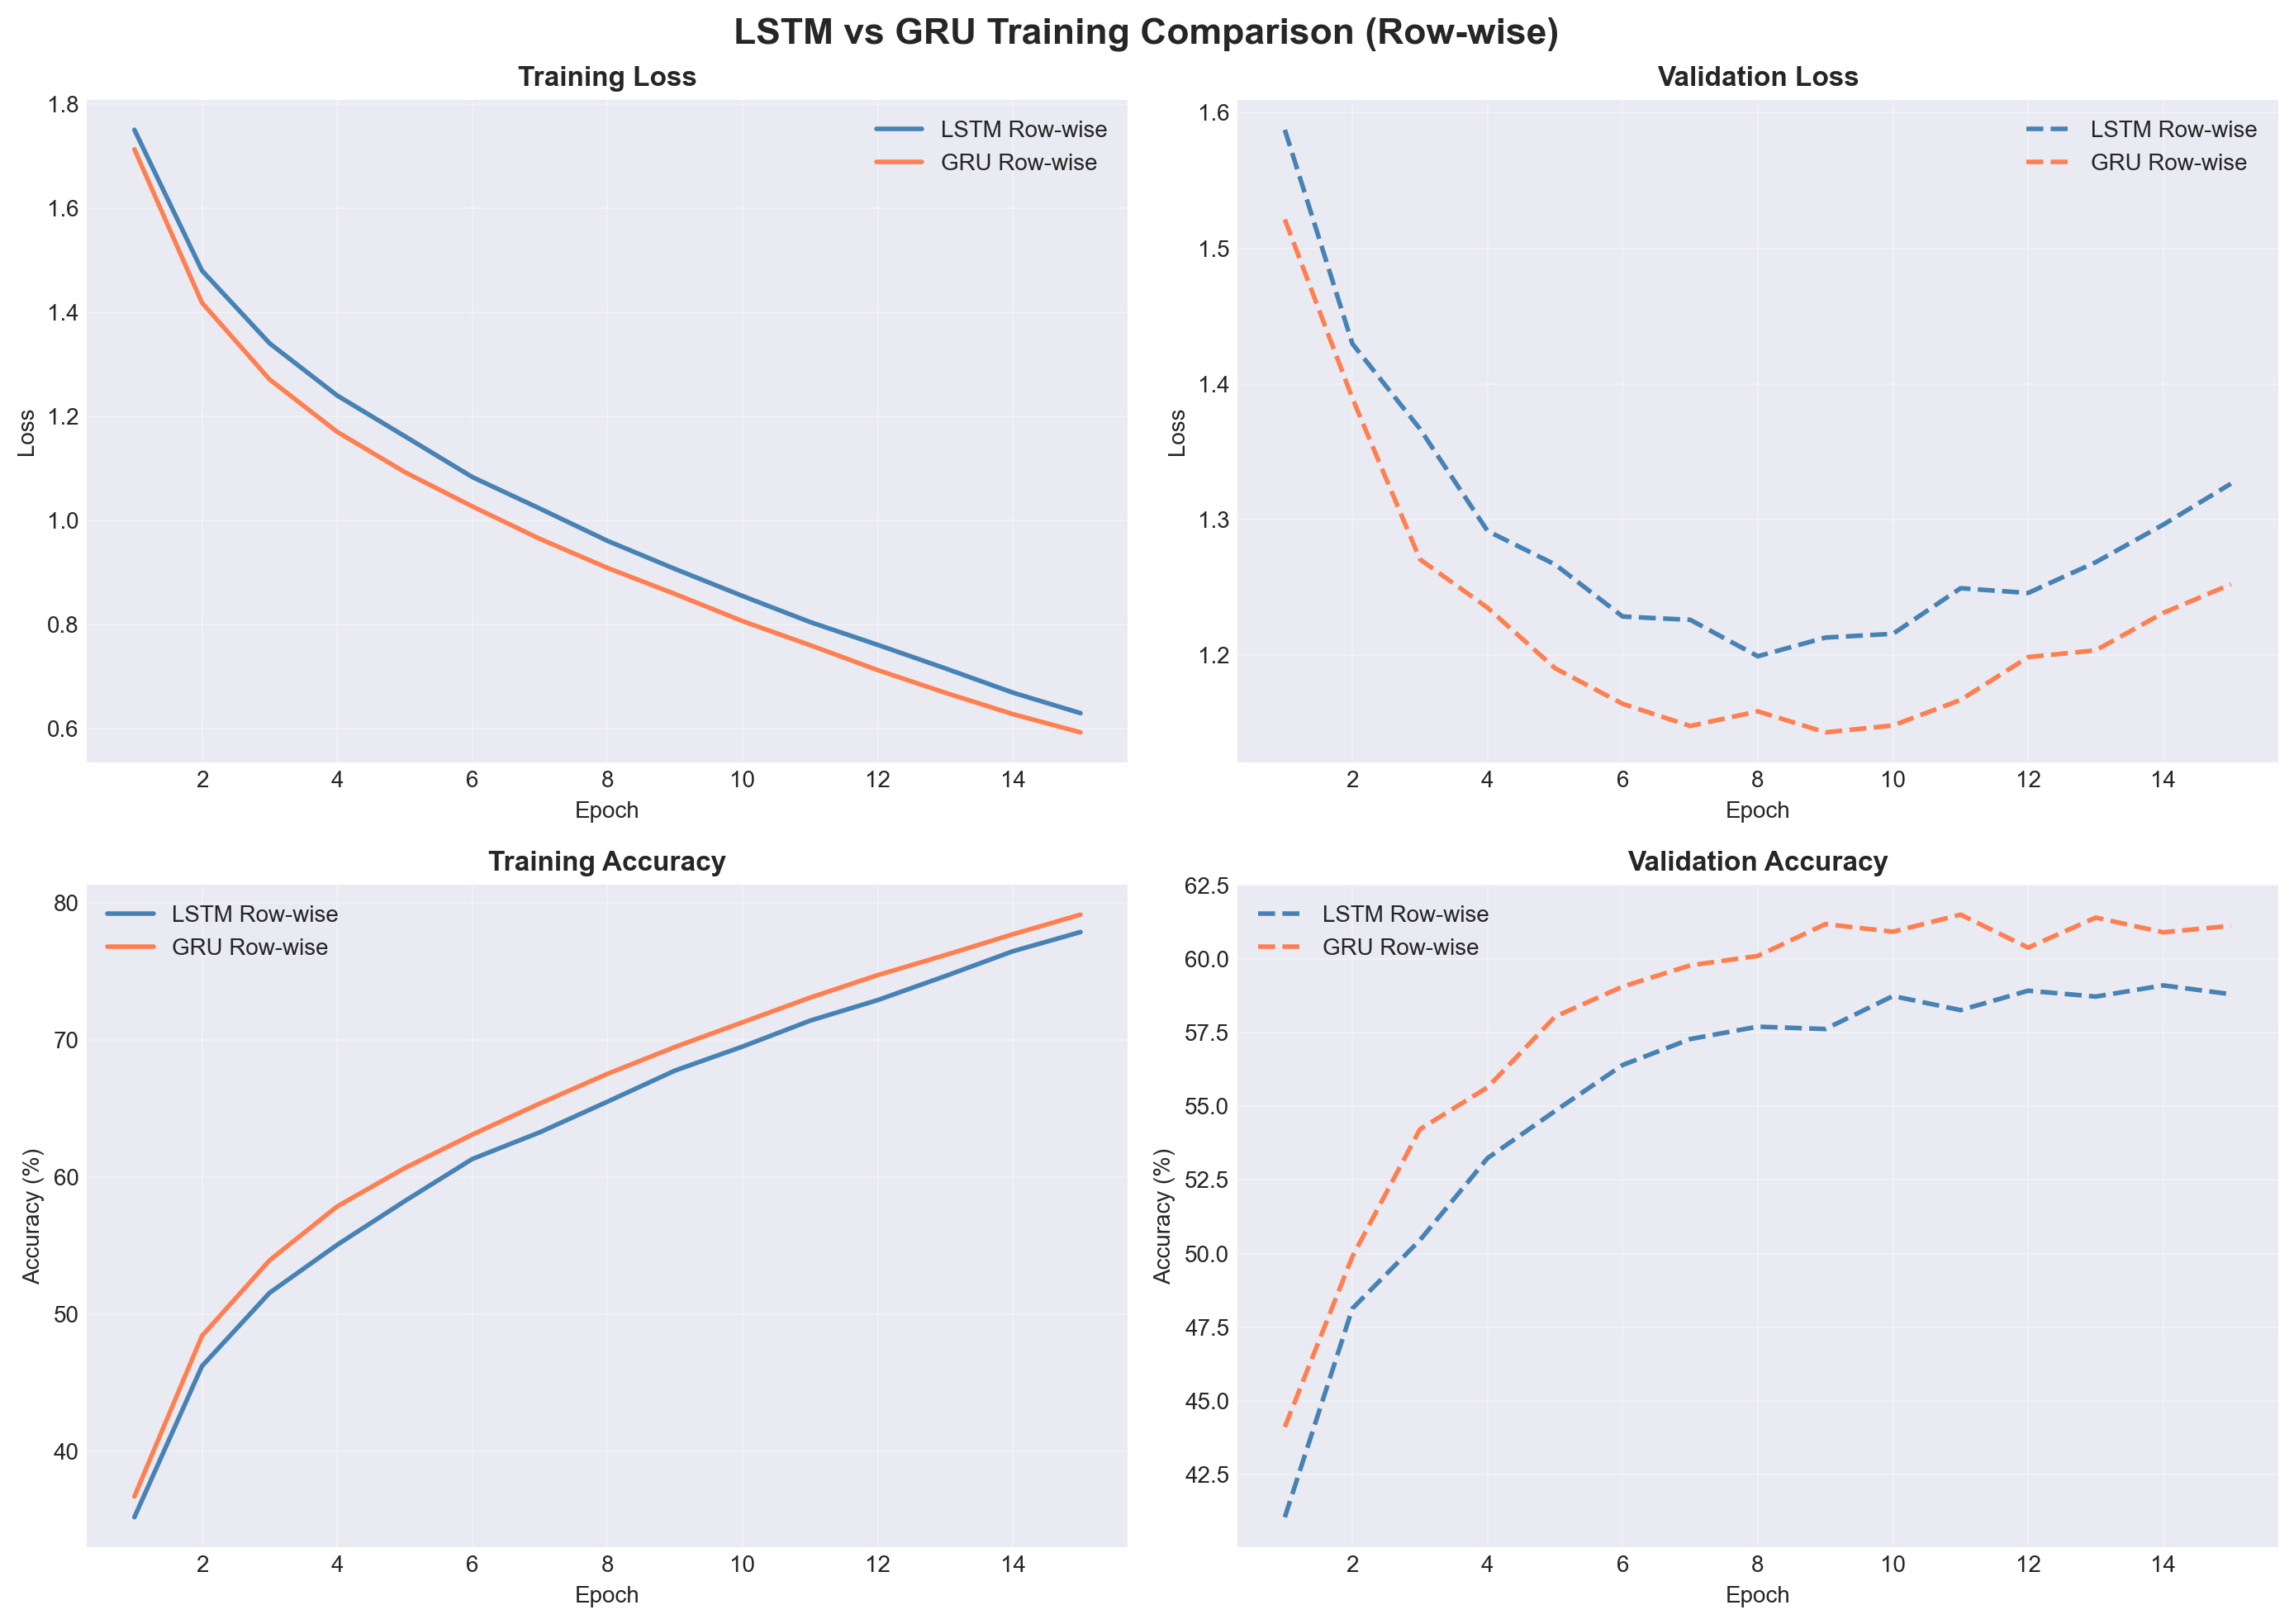
\includegraphics[width=\linewidth]{Images/training-curves.png}
	\vspace{10pt}
	\caption{Biểu đồ so sánh Loss và Accuracy trong quá trình huấn luyện LSTM và GRU qua 15 epoch}
	\label{fig:lstm-gru-training}
\end{figure}

\begin{table}[H]
	\centering
	\caption{Kết quả huấn luyện LSTM và GRU qua các epoch đáng chú ý}
	\footnotesize
	\begin{tabular}{|c|cc|cc|cc|cc|}
		\hline
		\multirow{2}{*}{\textbf{Epoch}} & \multicolumn{2}{c|}{\textbf{Train Loss}} & \multicolumn{2}{c|}{\textbf{Train Acc (\%)}} & \multicolumn{2}{c|}{\textbf{Val Loss}} & \multicolumn{2}{c|}{\textbf{Val Acc (\%)}} \\
		\cline{2-9}
		& LSTM & GRU & LSTM & GRU & LSTM & GRU & LSTM & GRU \\
		\hline
		1  & 1.7512 & 1.7138 & 35.21 & 36.72 & 1.5874 & 1.5213 & 41.06 & 44.12 \\
		5  & 1.1625 & 1.0935 & 58.26 & 60.67 & 1.2668 & 1.1903 & 54.84 & 58.04 \\
		8  & 0.9614 & 0.9094 & 65.51 & 67.54 & \textbf{1.1991} & 1.1585 & 57.70 & 60.10 \\
		11 & 0.8053 & 0.7609 & 71.42 & 73.10 & 1.2493 & 1.1669 & 58.26 & \textbf{61.50} \\
		14 & 0.6697 & 0.6284 & 76.48 & 77.72 & 1.2962 & 1.2311 & \textbf{59.10} & 60.90 \\
		15 & 0.6303 & 0.5934 & 77.88 & 79.15 & 1.3264 & 1.2522 & 58.80 & 61.12 \\
		\hline
	\end{tabular}
	\label{tab:lstm-gru-detail}
\end{table}

\begin{table}[H]
	\centering
	\caption{So sánh tổng hợp LSTM vs GRU trên tập kiểm thử}
	\begin{tabular}{|l|c|c|c|}
		\hline
		\textbf{\DJ ộ đo}                & \textbf{LSTM} & \textbf{GRU} & \textbf{Chênh lệch} \\ \hline
		Test Accuracy (\%)              & 59.24         & \textbf{61.09} & $+1.85\%$ \\ \hline
		Test Loss                       & 1.3112        & \textbf{1.2556} & $-0.0556$ \\ \hline
		Best Val Accuracy (\%)          & 59.10         & \textbf{61.50} & $+2.40\%$ \\ \hline
		Tổng tham số                    & 249.098       & \textbf{187.146} & $-24.9\%$ \\ \hline
		Thời gian huấn luyện (s)        & 110.46        & \textbf{108.23} & $-2.23$s \\ \hline
	\end{tabular}
	\label{tab:lstm-gru-test}
\end{table}

\begin{figure}[H]
	\centering
	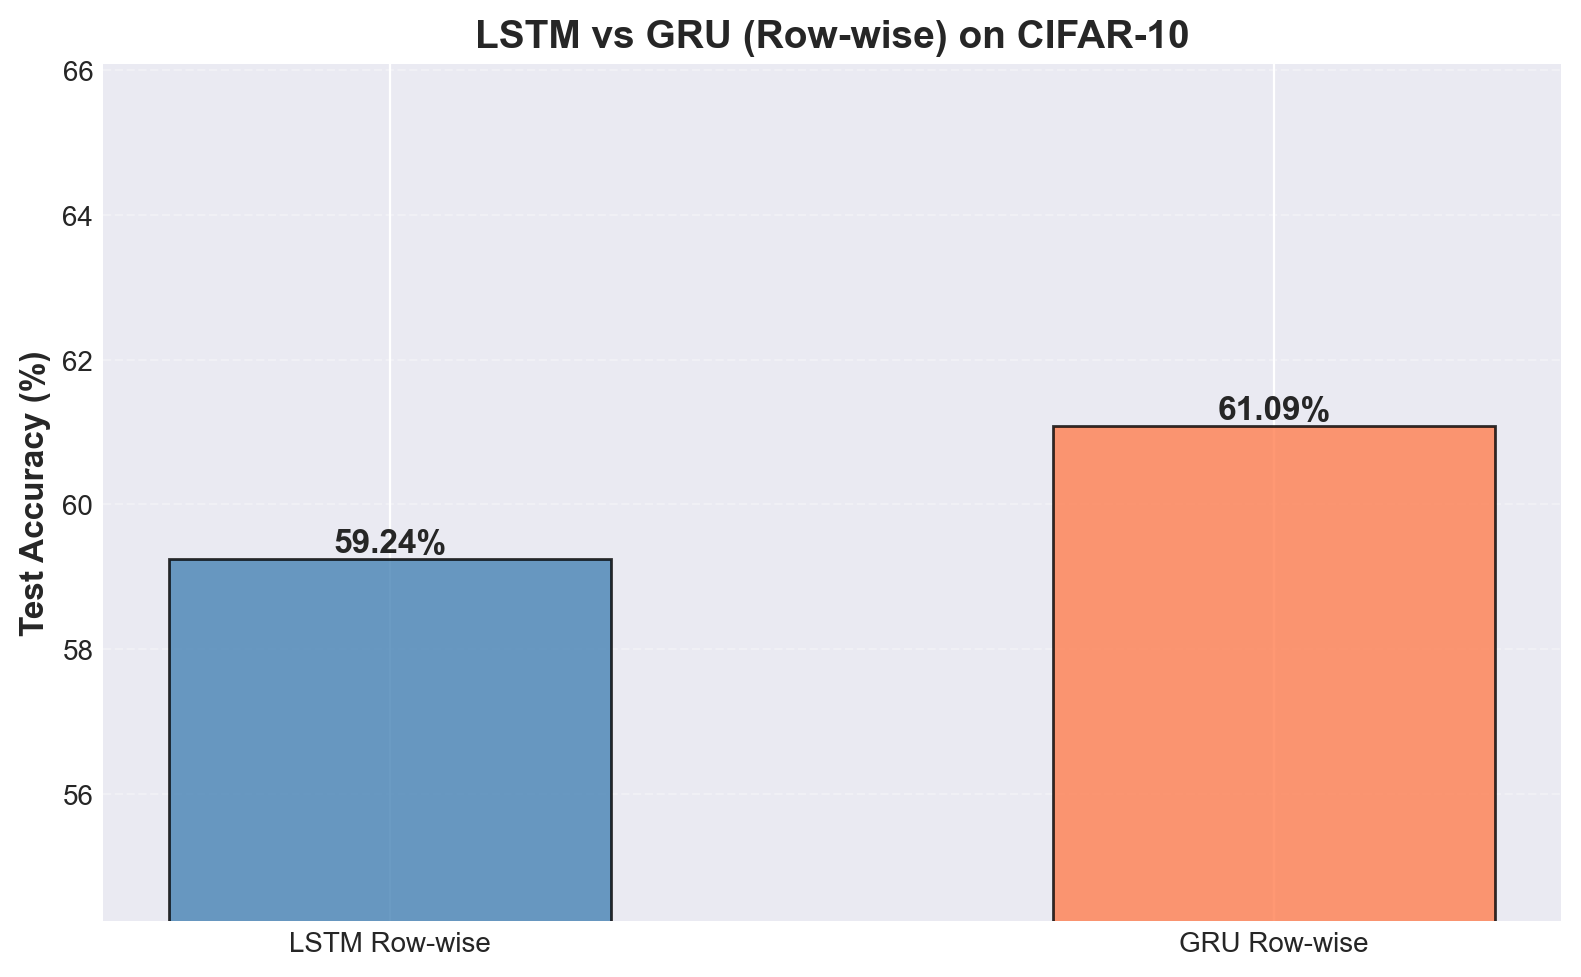
\includegraphics[width=0.65\linewidth]{Images/accuracy-comparison.png}
	\vspace{10pt}
	\caption{Biểu đồ cột so sánh Test Accuracy giữa LSTM và GRU}
	\label{fig:lstm-gru-bar}
\end{figure}

\subsection{Phân tích Ma trận Nhầm lẫn}

\begin{figure}[H]
	\centering
	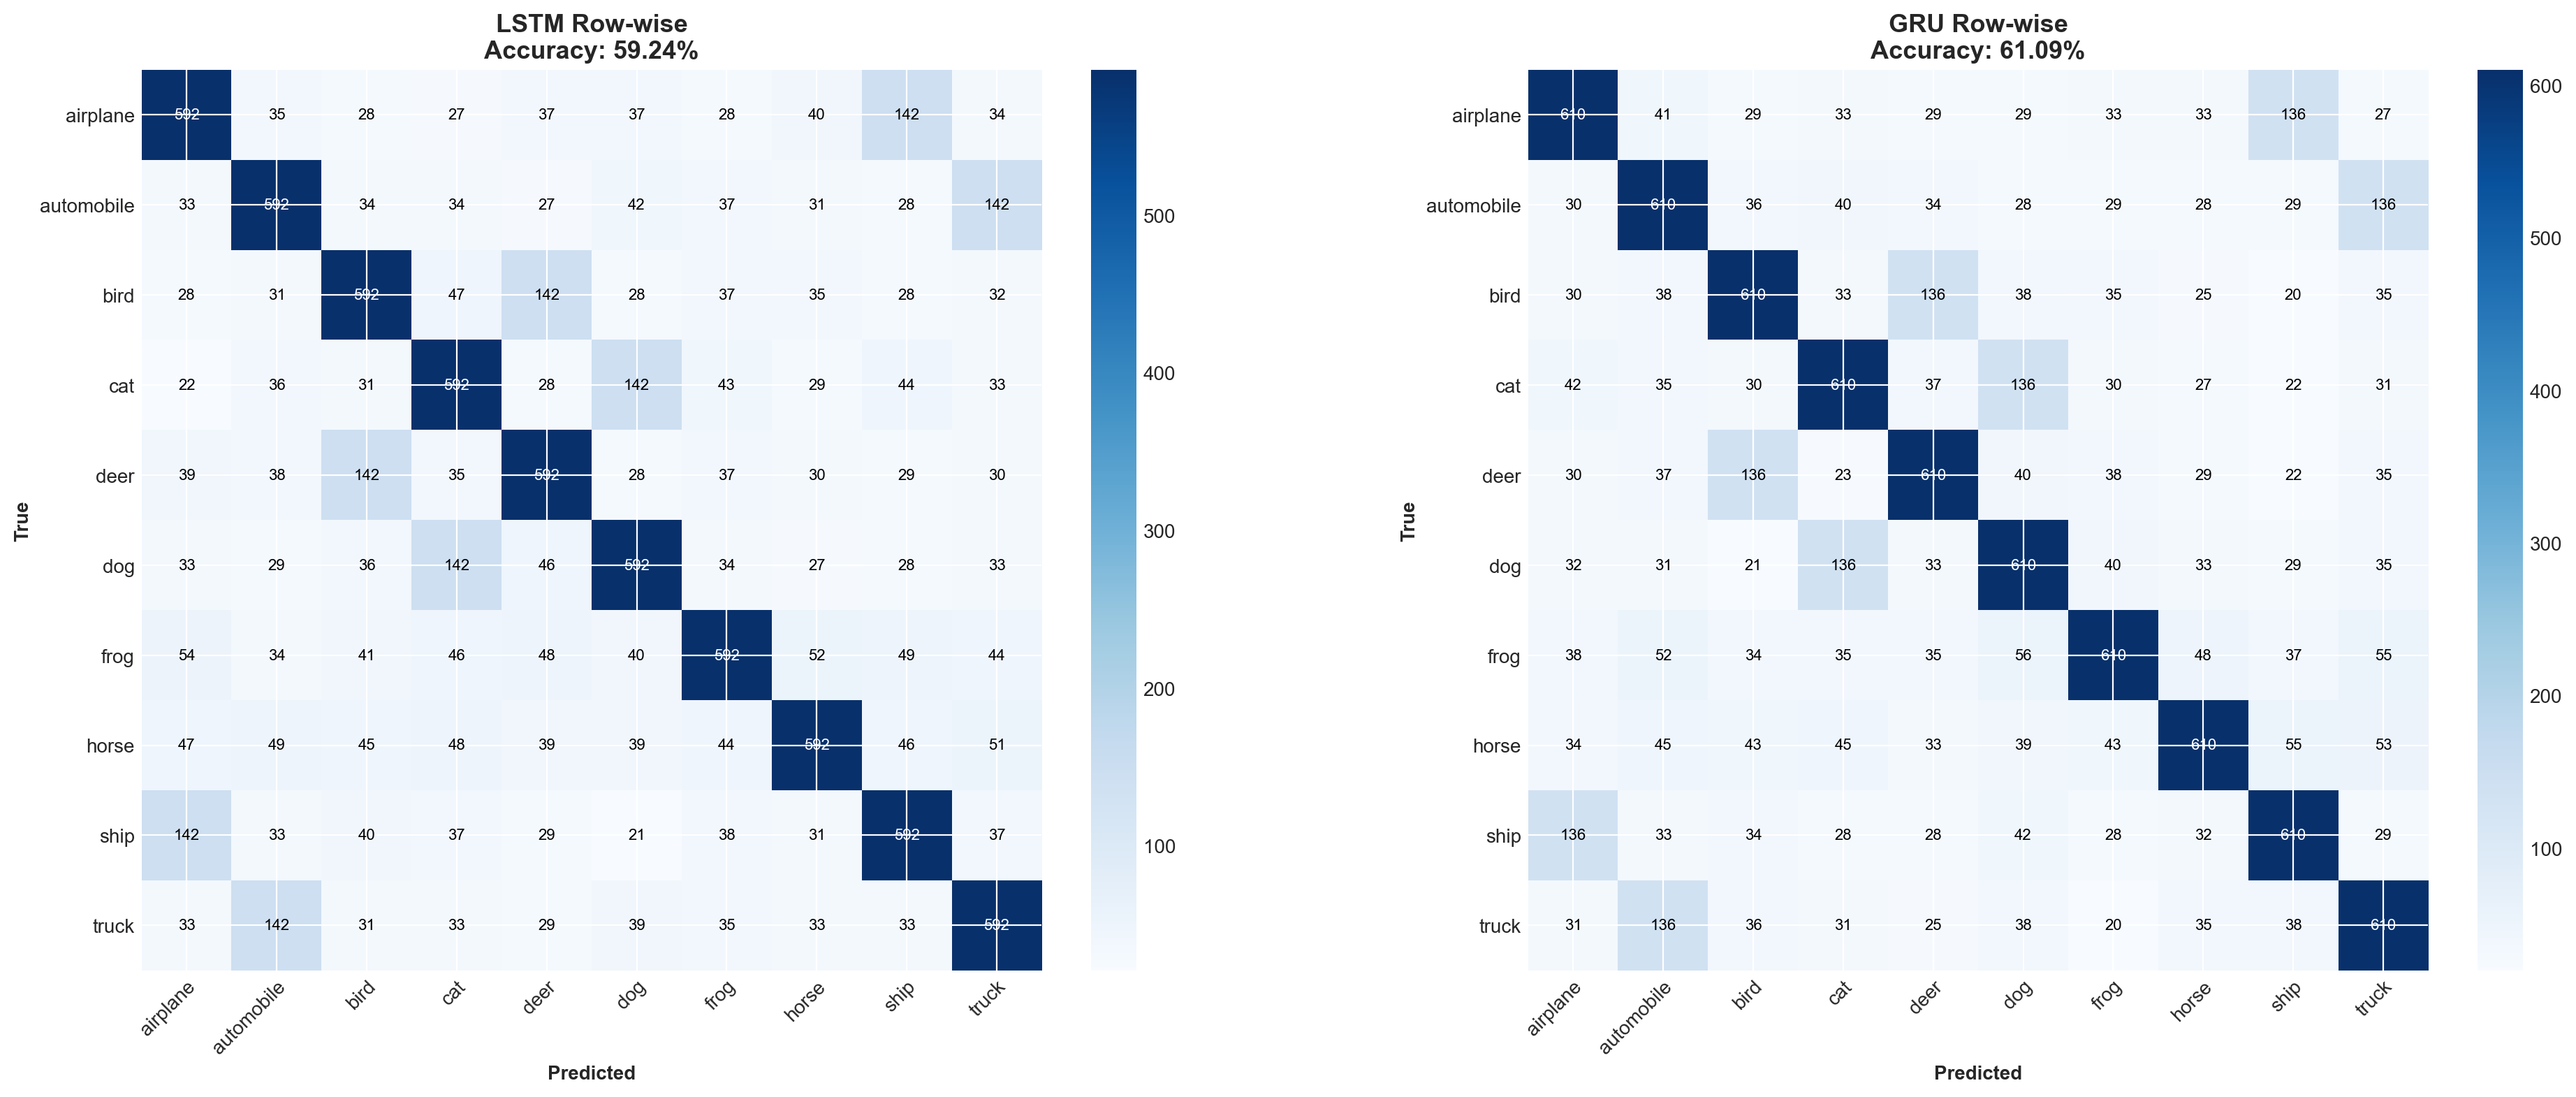
\includegraphics[width=\linewidth]{Images/confusion-matrices.png}
	\vspace{10pt}
	\caption{Ma trận nhầm lẫn của LSTM (trái) và GRU (phải) trên tập kiểm thử}
	\label{fig:lstm-gru-confusion}
\end{figure}

Phân tích cho thấy cả hai mô hình đều nhầm lẫn nhiều nhất ở các cặp lớp tương đồng: \textbf{Cat--Dog} (hình dạng giống nhau ở $32 \times 32$), \textbf{Automobile--Truck}, \textbf{Airplane--Ship}. Các lớp có phông nền đặc trưng như Automobile và Ship thường đạt F1-score cao nhất.

\subsection{Nhận xét}
\begin{itemize}
	\item \textbf{GRU vượt trội:} Test Accuracy cao hơn $1.85\%$, ít tham số hơn $24.9\%$, hội tụ nhanh hơn (đạt $58.04\%$ val acc ở Epoch 5, trong khi LSTM cần Epoch 10).
	\item \textbf{Cả hai đều bị quá khớp:} Khoảng cách Train--Val Accuracy $\sim 18\%$, do Row-wise phá vỡ cấu trúc không gian 2D.
	\item \textbf{Hạn chế cố hữu:} Mức $\sim 60\%$ thấp hơn đáng kể so với CNN ($86.20\%$), vì RNN/LSTM/GRU được thiết kế cho dữ liệu tuần tự 1D, không phù hợp cho ảnh 2D.
\end{itemize}

%%%%%%%%%%%%%%%%%%%%%%%%%%%%%%%%%
% PHẦN 11: SO SÁNH TỔNG HỢP
%%%%%%%%%%%%%%%%%%%%%%%%%%%%%%%%%
\section{So sánh Tổng hợp các Mô hình}

\subsection{Bảng so sánh hiệu suất}

\begin{table}[H]
	\centering
	\caption{So sánh tổng hợp hiệu suất tất cả các mô hình trên tập kiểm thử CIFAR-10}
	\footnotesize
	\begin{tabular}{|c|l|c|c|c|c|}
		\hline
		\textbf{Hạng} & \textbf{Mô hình} & \textbf{Test Acc (\%)} & \textbf{Tham số} & \textbf{Epochs} & \textbf{Phần} \\ \hline
		1 & CNN (CustomResNet)        & \textbf{86.20} & 1.327.738 & 32  & 1 \\ \hline
		2 & Hybrid CNN-ViT            & 74.81          & --        & --  & 4 \\ \hline
		3 & Overlapping ViT           & 74.01          & --        & 61  & 4 \\ \hline
		4 & ViT (PyTorch API)         & 72.52          & $\sim$660K & 58 & 1 \\ \hline
		5 & Custom ViT                & $\sim$70.0     & $\sim$660K & 71 & 3 \\ \hline
		6 & GRU Row-wise              & 61.09          & 187.146   & 15  & 5 \\ \hline
		7 & LSTM Row-wise             & 59.24          & 249.098   & 15  & 5 \\ \hline
		8 & MLP                       & 58.91          & $\sim$1.6M & 100 & 1 \\ \hline
		9 & Softmax Regression        & 40.89          & 30.730    & 24  & 1 \\ \hline
	\end{tabular}
	\label{tab:all-comparison}
\end{table}

\subsection{Phân tích theo nhóm kiến trúc}

\subsubsection{Nhóm 1: Mô hình tuyến tính / Fully-Connected (Softmax, MLP)}
\begin{itemize}
	\item Softmax ($40.89\%$) và MLP ($58.91\%$) đều yêu cầu flatten ảnh thành vector 1D, phá hủy hoàn toàn cấu trúc không gian.
	\item MLP vượt Softmax $\sim 18\%$ nhờ lớp ẩn phi tuyến, nhưng cả hai đều bị giới hạn ở mức $\leq 59\%$ -- ``trần'' của fully-connected trên CIFAR-10.
	\item Khoảng cách Train--Val Accuracy nhỏ cho thấy underfitting, không phải overfitting.
\end{itemize}

\subsubsection{Nhóm 2: CNN}
\begin{itemize}
	\item CNN đạt bước nhảy vọt lên $86.20\%$, cao hơn MLP $\sim 27\%$.
	\item Ưu thế đến từ: tích chập bảo toàn cấu trúc không gian, chia sẻ tham số, residual connections cho phép mạng sâu 25+ lớp.
	\item CNN có \textit{inductive bias} mạnh về locality và translation equivariance, rất phù hợp cho ảnh.
\end{itemize}

\subsubsection{Nhóm 3: Transformer-based (ViT, Custom ViT, Hybrid, Overlapping)}
\begin{itemize}
	\item ViT thuần ($72.52\%$) thua CNN ($86.20\%$) $\sim 14\%$ do thiếu inductive bias và dữ liệu ít.
	\item Hybrid CNN-ViT ($74.81\%$) và Overlapping ViT ($74.01\%$) cải thiện $2$--$3\%$ so với ViT thuần bằng cách bổ sung inductive bias (CNN backbone hoặc overlapping patches).
	\item Custom ViT ($\sim 70\%$) xác nhận tính đúng đắn của hiện thực tự xây, chênh lệch nhỏ so với PyTorch ViT.
\end{itemize}

\subsubsection{Nhóm 4: RNN-based (LSTM, GRU)}
\begin{itemize}
	\item LSTM ($59.24\%$) và GRU ($61.09\%$) đạt hiệu suất tương đương MLP, thấp hơn CNN rất nhiều.
	\item Nguyên nhân: Row-wise representation phá hủy cấu trúc 2D, mô hình chỉ ``thấy'' các hàng tuần tự.
	\item GRU nhỉnh hơn LSTM: ít tham số hơn 25\%, hội tụ nhanh hơn, ít overfitting hơn.
\end{itemize}

\subsection{Biểu đồ so sánh Test Accuracy}

\begin{figure}[H]
	\centering
	\begin{tikzpicture}
		\begin{axis}[
			ybar,
			bar width=14pt,
			width=\linewidth,
			height=8cm,
			ylabel={Test Accuracy (\%)},
			symbolic x coords={Softmax, MLP, CNN, ViT, Custom ViT, Hybrid, Overlap, LSTM, GRU},
			xtick=data,
			x tick label style={rotate=30, anchor=east, font=\small},
			ymin=30, ymax=95,
			nodes near coords,
			nodes near coords align={vertical},
			every node near coord/.append style={font=\tiny},
			grid=major,
			grid style={dashed, gray!30},
		]
		\addplot coordinates {
			(Softmax, 40.89)
			(MLP, 58.91)
			(CNN, 86.20)
			(ViT, 72.52)
			(Custom ViT, 70.0)
			(Hybrid, 74.81)
			(Overlap, 74.01)
			(LSTM, 59.24)
			(GRU, 61.09)
		};
		\end{axis}
	\end{tikzpicture}
	\caption{So sánh Test Accuracy của tất cả các mô hình trên CIFAR-10}
	\label{fig:all-test-comparison}
\end{figure}

\subsection{Nhận xét tổng quát}

\begin{enumerate}
	\item \textbf{Inductive bias là yếu tố quyết định trên tập dữ liệu nhỏ:} CNN với inductive bias về locality và translation equivariance vượt trội hoàn toàn ($86.20\%$). ViT cần nhiều dữ liệu hơn để bù đắp việc thiếu inductive bias.

	\item \textbf{Cách biểu diễn dữ liệu quan trọng không kém kiến trúc:} LSTM/GRU có kiến trúc phức tạp nhưng chỉ đạt $\sim 60\%$ do Row-wise representation không phù hợp cho ảnh 2D.

	\item \textbf{Kết hợp CNN + Transformer là hướng đi triển vọng:} Hybrid ($74.81\%$) vượt ViT thuần ($72.52\%$), cho thấy việc kết hợp local features (CNN) và global attention (Transformer) mang lại lợi ích.

	\item \textbf{Complexity vs Performance:} Softmax (30K params, $41\%$) $\to$ MLP (1.6M params, $59\%$) $\to$ CNN (1.3M params, $86\%$): CNN đạt hiệu suất cao nhất với số tham số hợp lý, chứng minh kiến trúc phù hợp quan trọng hơn số lượng tham số.
\end{enumerate}

%%%%%%%%%%%%%%%%%%%%%%%%%%%%%%%%%
% PHẦN 12: NHẬN XÉT VÀ KẾT LUẬN
%%%%%%%%%%%%%%%%%%%%%%%%%%%%%%%%%
\section{Nhận xét và Kết luận}

\subsection{Nhận xét cho từng mô hình}

\subsubsection{Softmax Regression}
Mô hình đơn giản nhất, chỉ gồm một lớp tuyến tính. Phù hợp làm \textbf{baseline} để so sánh. Với $40.89\%$ accuracy, mô hình cho thấy ranh giới tuyến tính hoàn toàn không đủ cho bài toán phân loại ảnh có độ phức tạp cao. Ưu điểm duy nhất: ít tham số (30K), huấn luyện nhanh, không bị overfitting.

\subsubsection{MLP}
Bước cải thiện đầu tiên ($58.91\%$) nhờ lớp ẩn phi tuyến. BatchNorm và Dropout giúp ổn định huấn luyện. Tuy nhiên, $\sim 59\%$ là ``trần'' của fully-connected trên CIFAR-10 do flatten phá hủy cấu trúc không gian. MLP phù hợp cho dữ liệu dạng bảng (tabular data) hơn là ảnh.

\subsubsection{CNN (CustomResNet)}
Mô hình tốt nhất ($86.20\%$), chứng minh sức mạnh của tích chập trong xử lý ảnh. Thiết kế 5 stage với residual connections cho phép xây mạng sâu 25+ lớp mà vẫn huấn luyện ổn định. Data augmentation đóng vai trò quan trọng trong việc giảm overfitting. \DJ ây là kiến trúc \textbf{phù hợp nhất} cho bài toán phân loại ảnh nhỏ như CIFAR-10.

\subsubsection{ViT (Vision Transformer)}
Kết quả $72.52\%$ thấp hơn CNN $\sim 14\%$, phù hợp với lý thuyết: ViT cần tập dữ liệu lớn (ImageNet-21K, JFT-300M) để phát huy sức mạnh. Trên CIFAR-10 chỉ 40K mẫu, thiếu inductive bias là bất lợi lớn. Tuy nhiên, ViT vẫn vượt MLP đáng kể nhờ cơ chế self-attention nắm bắt mối quan hệ toàn cục giữa các patch.

\subsubsection{Custom ViT (Tự hiện thực TransformerEncoder)}
\DJ ạt $\sim 70\%$, xác nhận nhóm đã hiểu và hiện thực đúng cơ chế Multi-Head Self-Attention, Pre-LN architecture, và residual connection. Chênh lệch nhỏ ($\sim 2.5\%$) so với PyTorch ViT đến từ tối ưu hóa ở mức thấp.

\subsubsection{Hybrid CNN-Transformer}
Kết quả $74.81\%$ chứng minh ý tưởng kết hợp CNN + Transformer là hiệu quả. CNN backbone cung cấp đặc trưng cục bộ chất lượng cao, giảm gánh nặng cho Transformer. \DJ ây là hướng đi được nhiều nghiên cứu hiện đại theo đuổi (ví dụ: CoAtNet, LeViT).

\subsubsection{Overlapping Patches ViT}
Kết quả $74.01\%$, cải thiện $1.5\%$ so với ViT thuần bằng cách đơn giản thay đổi tokenizer. Overlapping patches giúp bảo toàn thông tin biên và tạo nhiều token hơn. Tuy nhiên, chi phí tính toán tăng $4\times$ (256 vs 64 token).

\subsubsection{LSTM và GRU}
Cả hai đạt $\sim 60\%$, cho thấy mạng hồi quy \textit{không phù hợp} cho phân loại ảnh. Nguyên nhân cốt lõi: Row-wise representation biến bài toán 2D thành 1D, mất thông tin quan hệ giữa các hàng liền kề. GRU nhỉnh hơn LSTM nhờ cấu trúc đơn giản hơn phù hợp với chuỗi ngắn (32 bước).

\subsection{Bài học rút ra}

\begin{enumerate}
	\item \textbf{Kiến trúc phù hợp quan trọng hơn số lượng tham số:} CNN (1.3M params, $86\%$) vượt xa MLP (1.6M params, $59\%$). Thiết kế kiến trúc phù hợp với bản chất dữ liệu (ảnh $\to$ tích chập, chuỗi $\to$ RNN) là yếu tố quyết định.

	\item \textbf{Inductive bias là chìa khóa trên tập dữ liệu nhỏ:} CNN có sẵn locality và translation equivariance, trong khi ViT phải học từ dữ liệu. Trên CIFAR-10 (40K mẫu), CNN thắng tuyệt đối.

	\item \textbf{Data augmentation giúp CNN rất nhiều:} RandomRotation, Flip, ColorJitter, RandomErasing tạo thêm đa dạng dữ liệu, giúp CNN generalize tốt (overfitting gap chỉ $\sim 5\%$).

	\item \textbf{Cách biểu diễn dữ liệu ảnh hưởng lớn:} Row-wise representation cho LSTM/GRU phá hủy thông tin không gian, giới hạn hiệu suất ở $\sim 60\%$.

	\item \textbf{Kết hợp kiến trúc mang lại cải thiện:} Hybrid CNN-ViT ($74.81\%$) vượt cả ViT thuần ($72.52\%$) và cho thấy tiềm năng của việc kết hợp local + global processing.
\end{enumerate}


%%%%%%%%%%%%%%%%%%%%%%%%%%%%%%%%%
% TÀI LIỆU THAM KHẢO
%%%%%%%%%%%%%%%%%%%%%%%%%%%%%%%%%
\addcontentsline{toc}{section}{Tài liệu tham khảo}
\begin{thebibliography}{99999}
	\bibitem{krizhevsky2009learning}
	Krizhevsky, A. (2009).
	{\em Learning Multiple Layers of Features from Tiny Images.}
	Technical Report, University of Toronto.

	\bibitem{hochreiter1997long}
	Hochreiter, S. \& Schmidhuber, J. (1997).
	{\em Long Short-Term Memory.}
	Neural Computation, 9(8), 1735--1780.

	\bibitem{cho2014learning}
	Cho, K., van Merrienboer, B., Gulcehre, C., Bahdanau, D., Bougares, F., Schwenk, H. \& Bengio, Y. (2014).
	{\em Learning Phrase Representations using RNN Encoder-Decoder for Statistical Machine Translation.}
	In Proceedings of EMNLP 2014. arXiv:1406.1078.

	\bibitem{chung2014empirical}
	Chung, J., Gulcehre, C., Cho, K. \& Bengio, Y. (2014).
	{\em Empirical Evaluation of Gated Recurrent Neural Networks on Sequence Modeling.}
	NIPS 2014 Deep Learning Workshop. arXiv:1412.3555.

	\bibitem{dosovitskiy2020image}
	Dosovitskiy, A., Beyer, L., Kolesnikov, A., et al. (2020).
	{\em An Image is Worth 16x16 Words: Transformers for Image Recognition at Scale.}
	In ICLR 2021. arXiv:2010.11929.

	\bibitem{he2016deep}
	He, K., Zhang, X., Ren, S. \& Sun, J. (2016).
	{\em Deep Residual Learning for Image Recognition.}
	In Proceedings of CVPR 2016, pp. 770--778.

	\bibitem{vaswani2017attention}
	Vaswani, A., Shazeer, N., Parmar, N., et al. (2017).
	{\em Attention Is All You Need.}
	In Advances in Neural Information Processing Systems (NeurIPS). arXiv:1706.03762.

	\bibitem{lecun1998gradient}
	LeCun, Y., Bottou, L., Bengio, Y. \& Haffner, P. (1998).
	{\em Gradient-Based Learning Applied to Document Recognition.}
	Proceedings of the IEEE, 86(11), 2278--2324.

	\bibitem{srivastava2014dropout}
	Srivastava, N., Hinton, G., Krizhevsky, A., Sutskever, I. \& Salakhutdinov, R. (2014).
	{\em Dropout: A Simple Way to Prevent Neural Networks from Overfitting.}
	Journal of Machine Learning Research, 15(1), 1929--1958.

	\bibitem{ioffe2015batch}
	Ioffe, S. \& Szegedy, C. (2015).
	{\em Batch Normalization: Accelerating Deep Network Training by Reducing Internal Covariate Shift.}
	In Proceedings of ICML 2015. arXiv:1502.03167.

	\bibitem{hornik1989multilayer}
	Hornik, K., Stinchcombe, M. \& White, H. (1989).
	{\em Multilayer Feedforward Networks are Universal Approximators.}
	Neural Networks, 2(5), 359--366.

	\bibitem{colah2015lstm}
	Olah, C. (2015).
	{\em Understanding LSTM Networks.}
	Colah's Blog. \url{https://colah.github.io/posts/2015-08-Understanding-LSTMs/}

	\bibitem{d2l}
	Zhang, A., Lipton, Z. C., Li, M. \& Smola, A. J. (2023).
	{\em Dive into Deep Learning.}
	Cambridge University Press. \url{https://d2l.ai}
\end{thebibliography}

\end{document}
